%% DC 10: The first analysis has to be longer, and walk us through in more detail, than the other analyses.  I think it's a full section in its own right.
\section{Cohorts matter: Variation in activity, effort, survival}

In this section, we will use a common metric of user activity in online communities, the number of posts per user, to show how two main time-aware approaches to analyzing behavior provide additional insights beyond simple chronological aggregation.  The first approach uses a notion of time relative to an event of interest (such as a user's first post); the second focuses on cohort effects.

\subsection{The Aggregate View of Users' Activity}

%\begin{figure}[!tb]
%\centering
%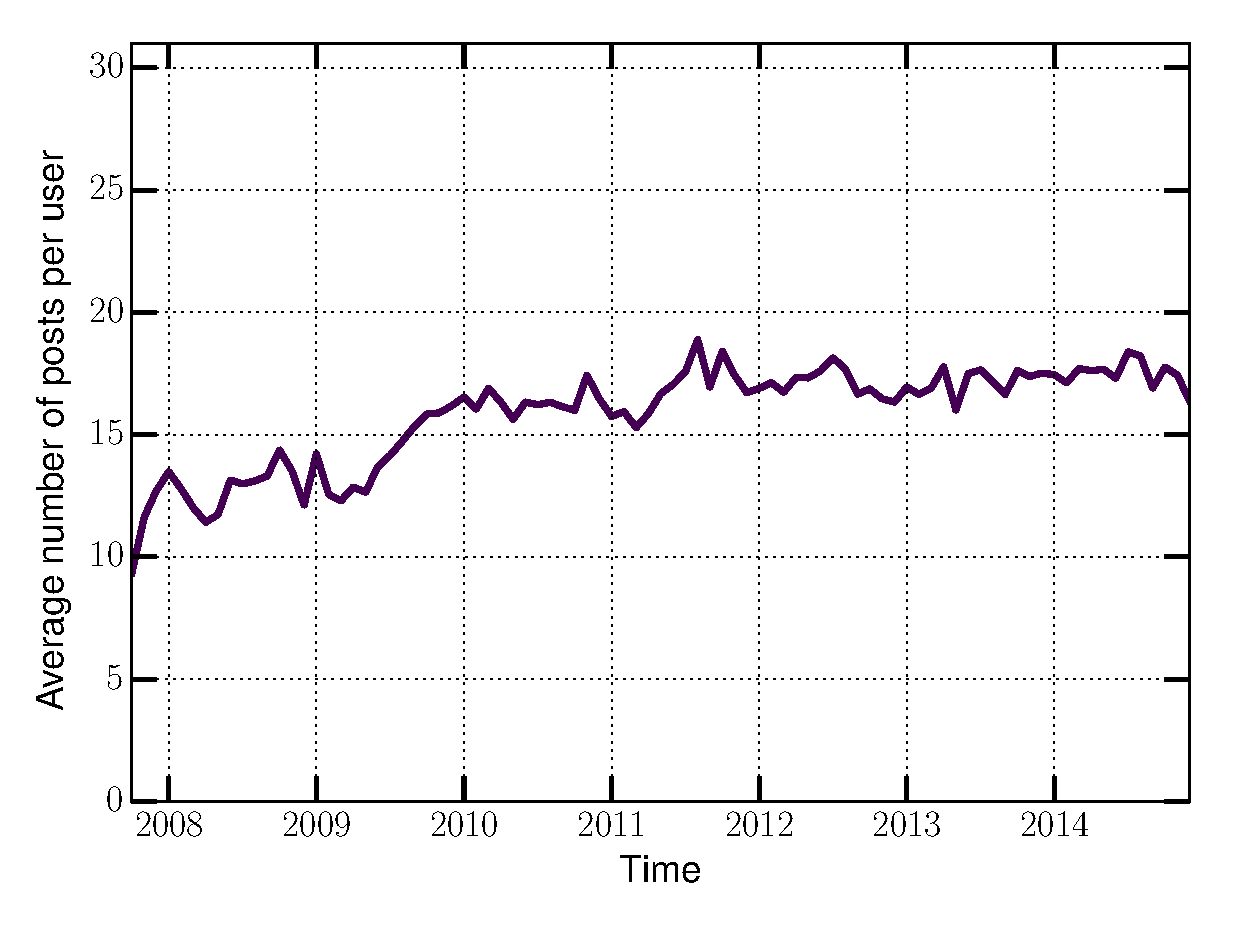
\includegraphics[scale=0.4]{./images/avr_posts_per_user_over_time_total.eps}
%\caption{Monthly average of posts per active users over time. Posts as either comments or submissions, we count the total sum of comments and submissions for each month. Active users are the ones that made at least one post in the said month. }
%\label{fig:avr_posts_per_user_over_time_total}
%\end{figure}

\begin{figure}[!tb]
\centering
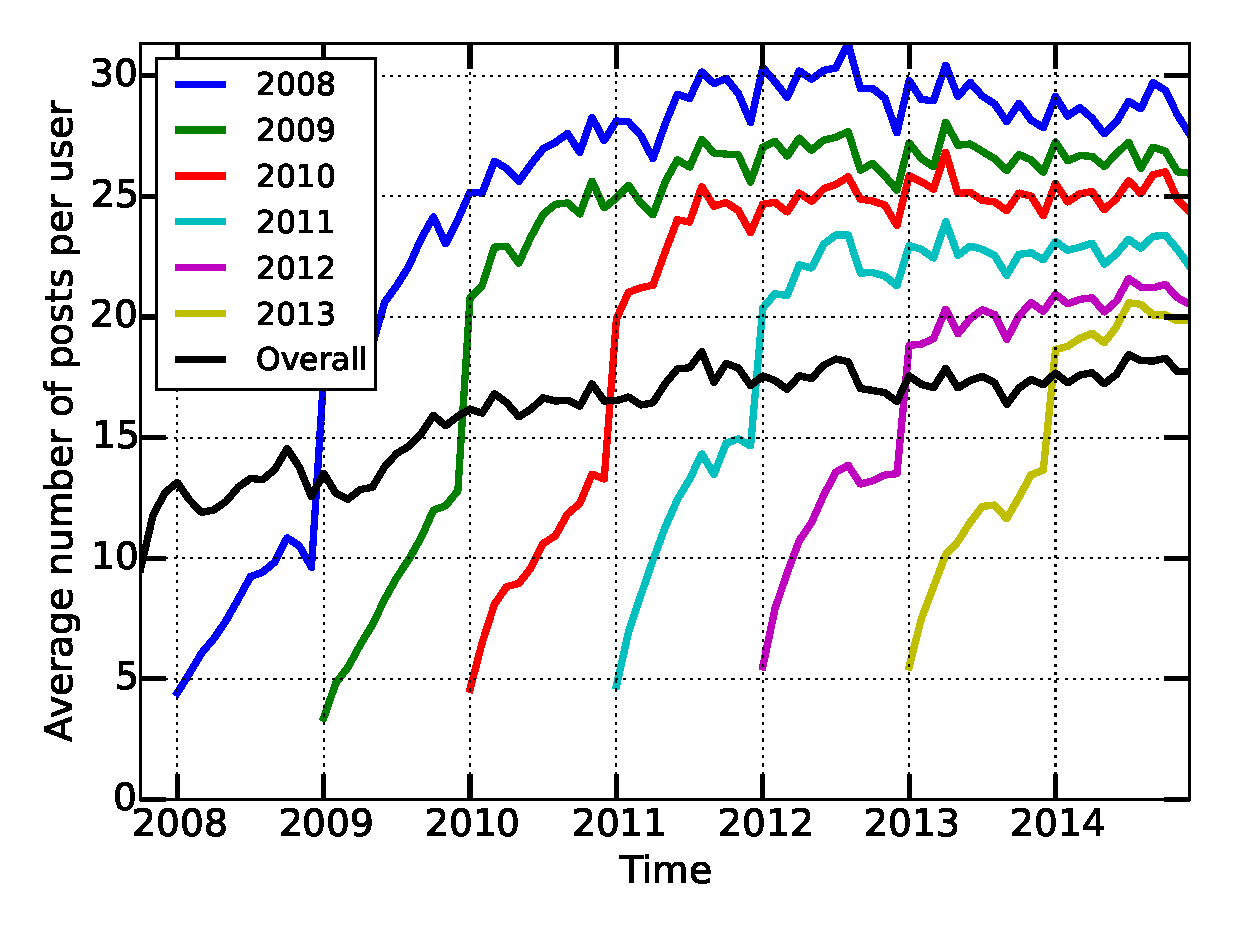
\includegraphics[scale=0.4]{./images/avr_posts_per_user_over_time_cohorts.eps}
\caption{Average number of posts per active users for the overall network and segmented by the user creation year. Posts as either comments or submissions, we count the total sum of comments and submissions for each month. Active users are the ones that made at least one post in the said month. The user creation year is defined as the year the user made his/her first post. The averages over the cohort year is lower because users are constantly being created over the year. Once you move past the cohort year, the user creation halts (including the high number of ``throw away accounts'') and we only observe the ``death'' of users, that has a strong impact in the count of users for the average, therefore the significant discontinuity by the end of the cohort year. Here we observe that different years level in different values for posts per user, having older users posting more than younger users as a general trend. We also observe that the overall average levels at a lower value than the cohorts also for the fact that it takes into consideration the users that are being created at all points.}
\label{fig:avr_posts_per_user_over_time_cohorts}
\end{figure}

Figure~\ref{fig:avr_posts_per_user_over_time_cohorts} shows the average number of posts (submissions plus comments) per month by users who were active in that month.  Taken at face value, this suggests that over the first few years of Reddit, users became more active in posting and that per-user activity has remained more or less steady since mid-2011.

\subsection{Activity relative to a user's lifespan}

%% DC 10: This is the new figure, the one that's adjusted to be relative to user creation date like Figure 5 but aggreated over all users rather than separated by cohort.

%% DC 10: This is my best guess as to what the aggregate version of the avr_posts_per_user_cohorts figure looks like
This average view hides several important aspects of users' activity dynamics.  In Figure~\ref{fig:avr_posts_per_user_cohorts_relative}, we show a different view that emphasizes the trajectory over a user's lifespan.  Here, we scale the x-axis not by clock time, as in the prior figure, but by time since the user's first post: ``1'' on the x-axis refers to one year since the user's account creation, and so on.  
One caution about interpreting the graphs that are relative to the user's start time is that the amount of data available rapidly decreases over time, meaning that values toward the right side of an individual data series are more subject to individual variation.  
%% DC 10: The way to really handle this would probably be confidence intervals, but we should at least note it somewhere and this is the best way I could think of for now.

This figure shows that a user's tenure matters: the longer a user survives, the more posts they make over time.  Interestingly, we see that the curve rises much higher than it does in Figure~\ref{avr_posts_per_user_over_time_total}: users who survive over five years have almost 50\% more posts per year than average. 

\subsection{Cohort-based views of posting activity}

%\begin{figure}[!tb]
%\centering
%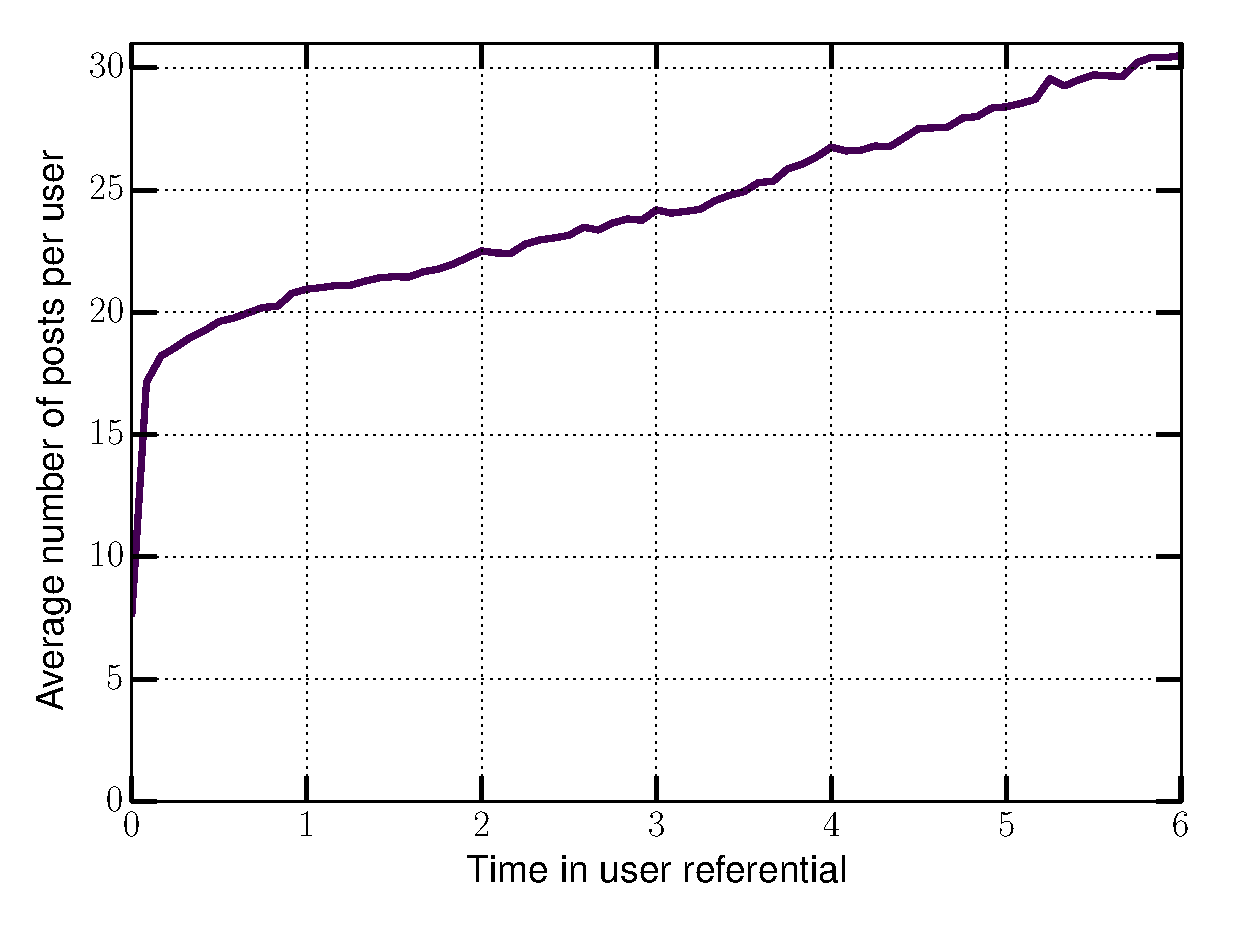
\includegraphics[scale=0.4]{./images/avr_posts_per_user_user_ref_total.eps}
%\caption{Evolution of all users in reddit. The x-axis is the time from the user creation referential, i.e., each message creation time is measured in terms of when the user was created. Each tick is one year and we discretized time by month --- the n-th bin holds messages the user wrote in the n-th month. The user count for each month is the number of users that were active, that is, the users that authored at least one post in their n-th month. Since we are looking at the user time referential, you can understand this as the surviving users after x time. The y-axis is the number of posts per active users. }
%\label{fig:avr_posts_per_user_user_ref_total}
%\end{figure}

\begin{figure}[!tb]
\centering
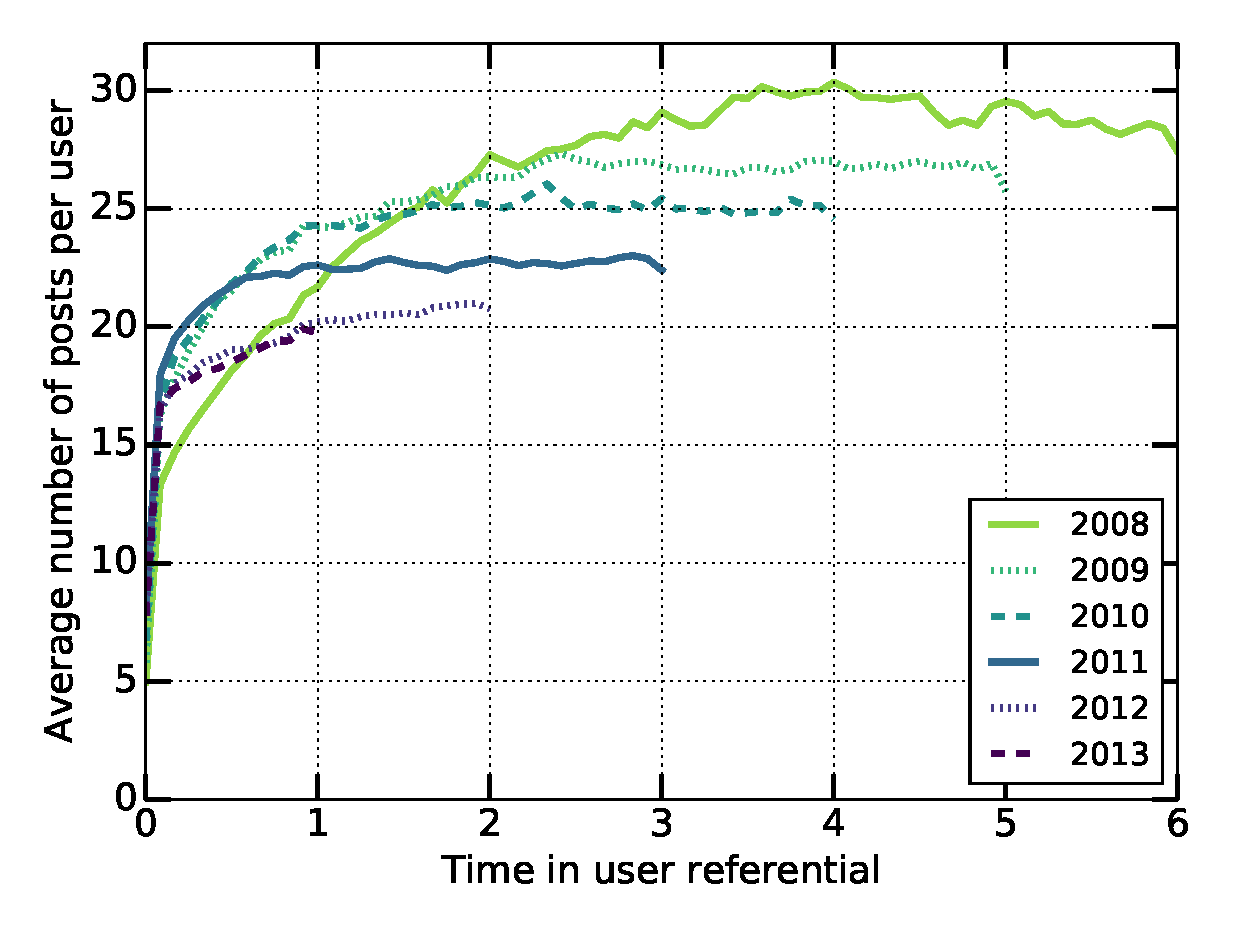
\includegraphics[scale=0.4]{./images/avr_posts_per_user_cohorts.eps}
\caption{Number of posts per active user for  the overall set of users and cohorts on the user creation date. The x-axis is the time from the user creation referential, i.e., each message creation time is measured in terms of when the user was created. Each tick is one year and we discretized time by month --- the n-th bin holds messages the user wrote in the n-th month. Since we are looking at the user time referential, you can understand this as the surviving users after x time. An interpretation of this says ``users that survived x time are posting on average y messages''. Here we see that, although the 2008 cohort level at a higher value, the evolution of the number of posts took a longer time to increase. The other cohorts seem to follow a more regular pattern after the first year: older users that survived the first year post more on average than younger users that survived the first year. Since we are talking about surviving users, it is not clear from this figure whether these curves increase because the ``low posting users'' are dying earlier or because the users are actually increasing their activity as they live on. To differentiate these cases, Figure \ref{fig:avr_posts_per_user_for_surviving_year} shows, for each cohort, the average posting for users grouped by the number of years they survived in the cohort.}
\label{fig:avr_posts_per_user_cohorts_relative}
\end{figure}

\begin{figure}[!tb]
\centering
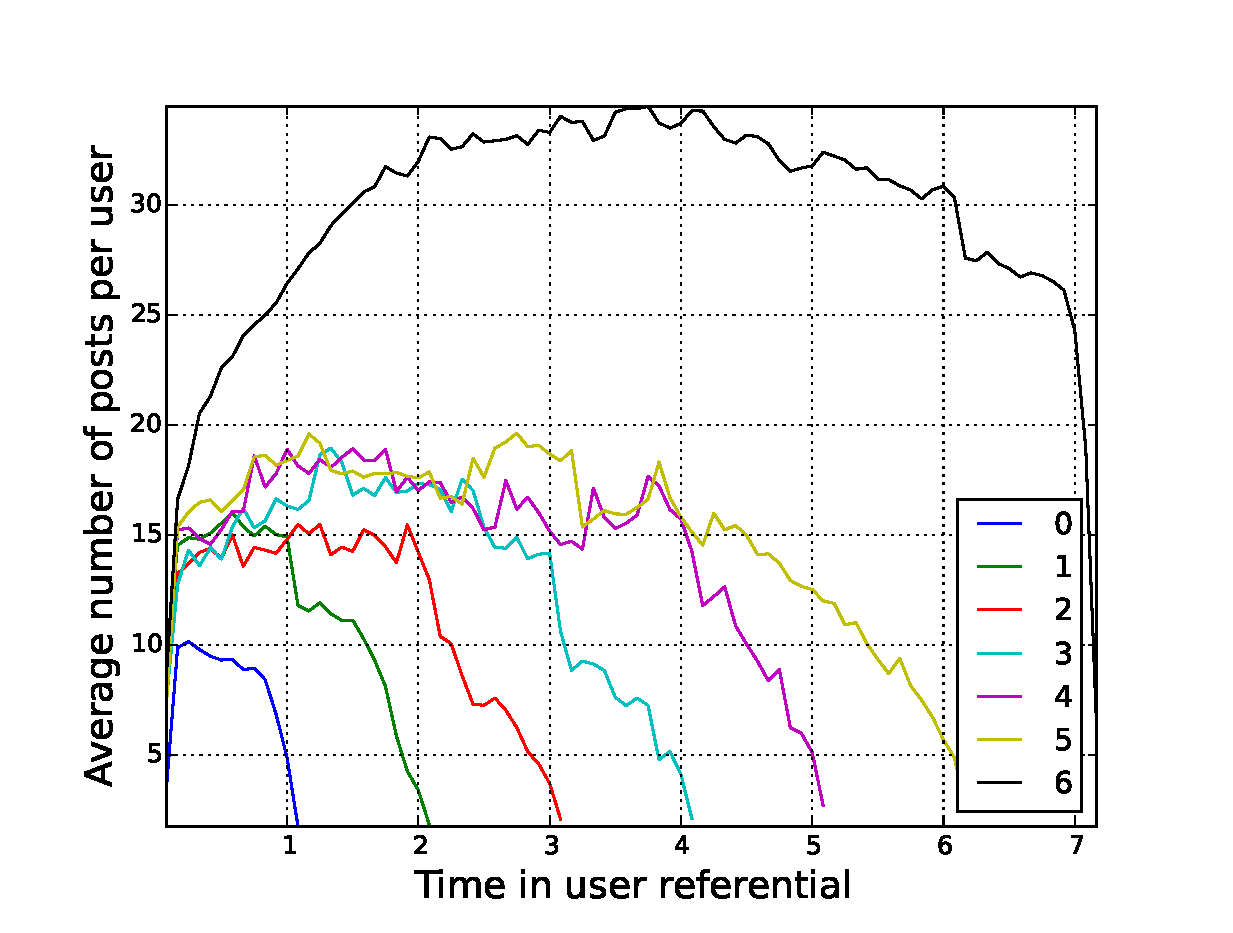
\includegraphics[scale=0.2]{./images/avr_posts_per_user_for_surviving_year_for_2008.eps}
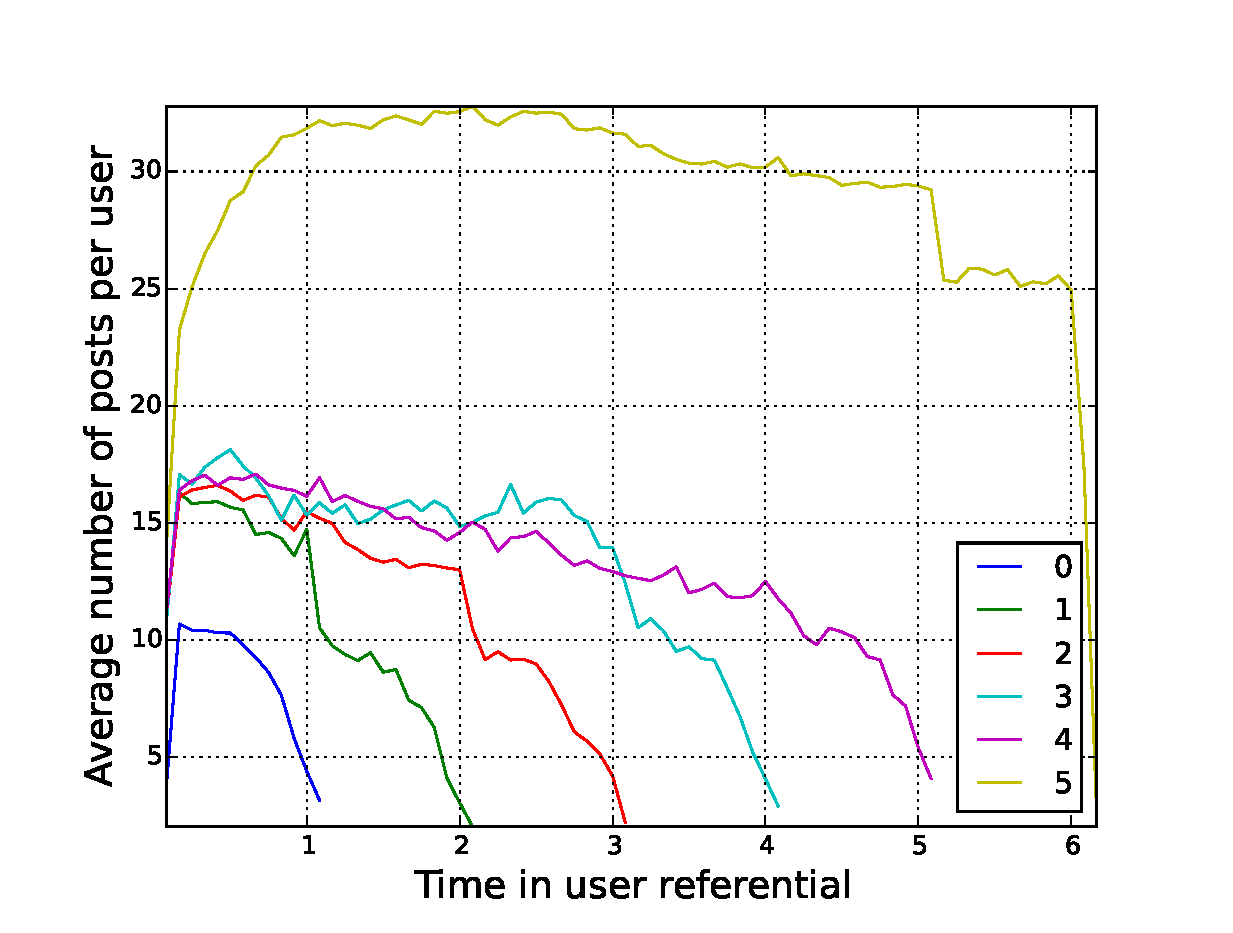
\includegraphics[scale=0.2]{./images/avr_posts_per_user_for_surviving_year_for_2009.eps}
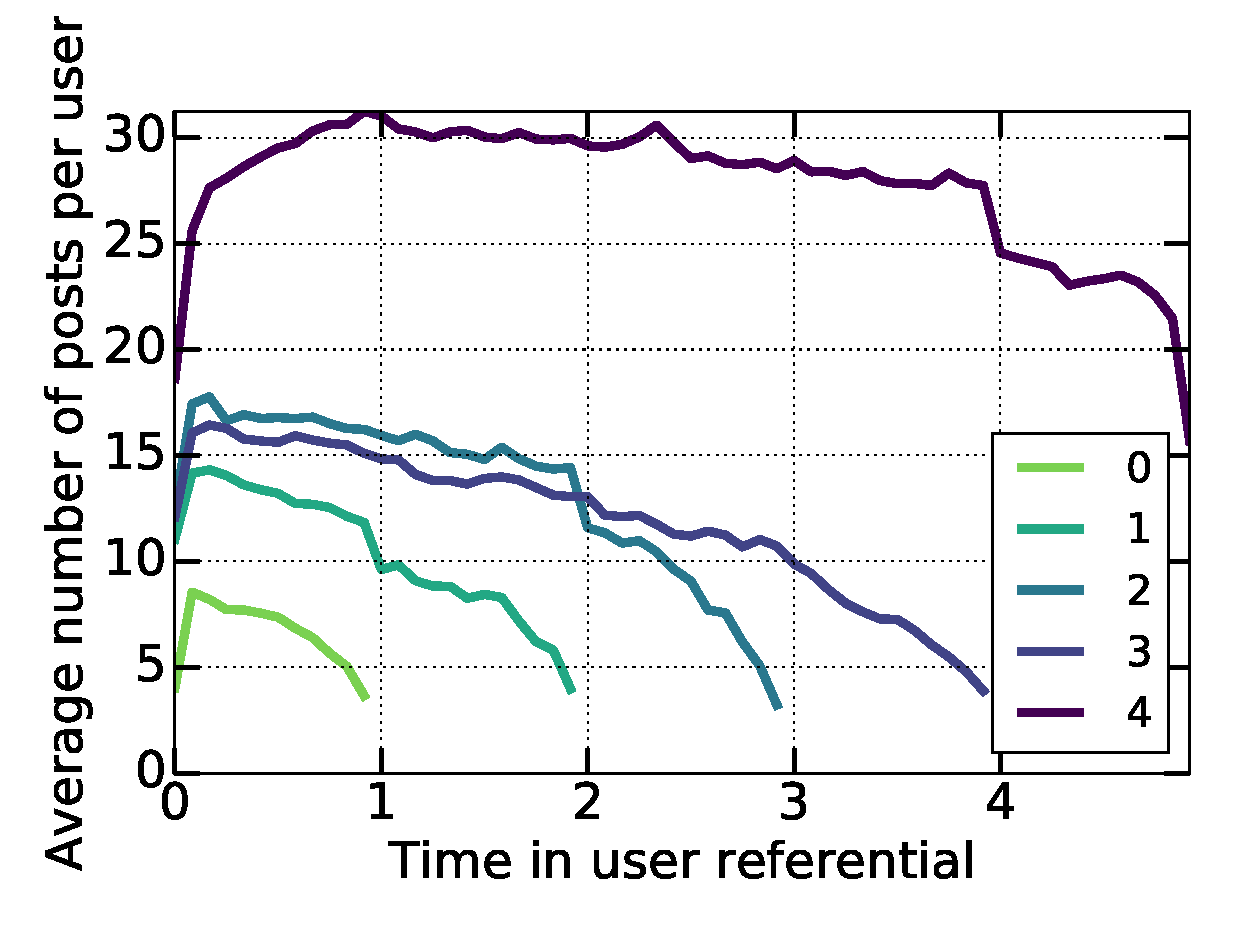
\includegraphics[scale=0.2]{./images/avr_posts_per_user_for_surviving_year_for_2010.eps}
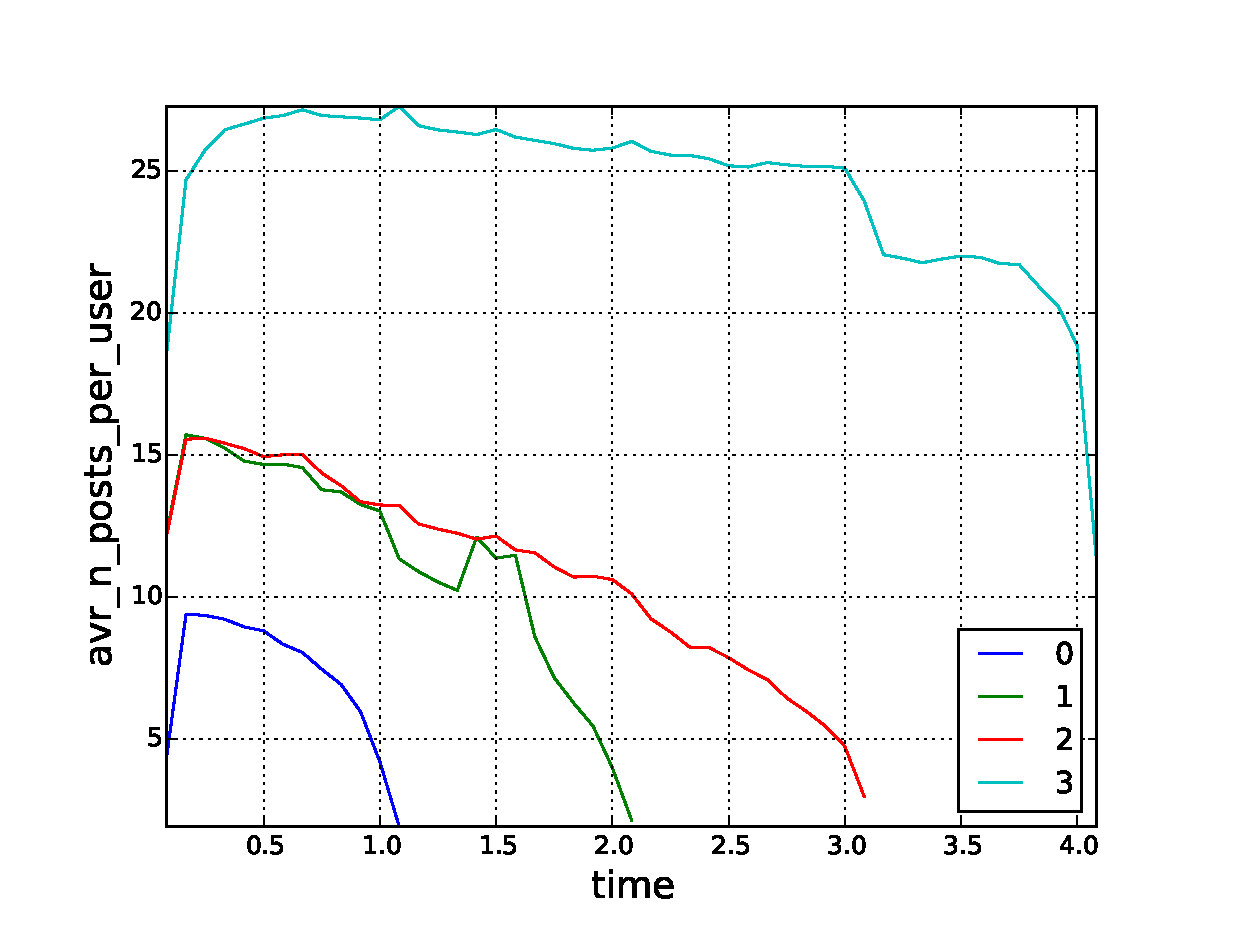
\includegraphics[scale=0.2]{./images/avr_posts_per_user_for_surviving_year_for_2011.eps}
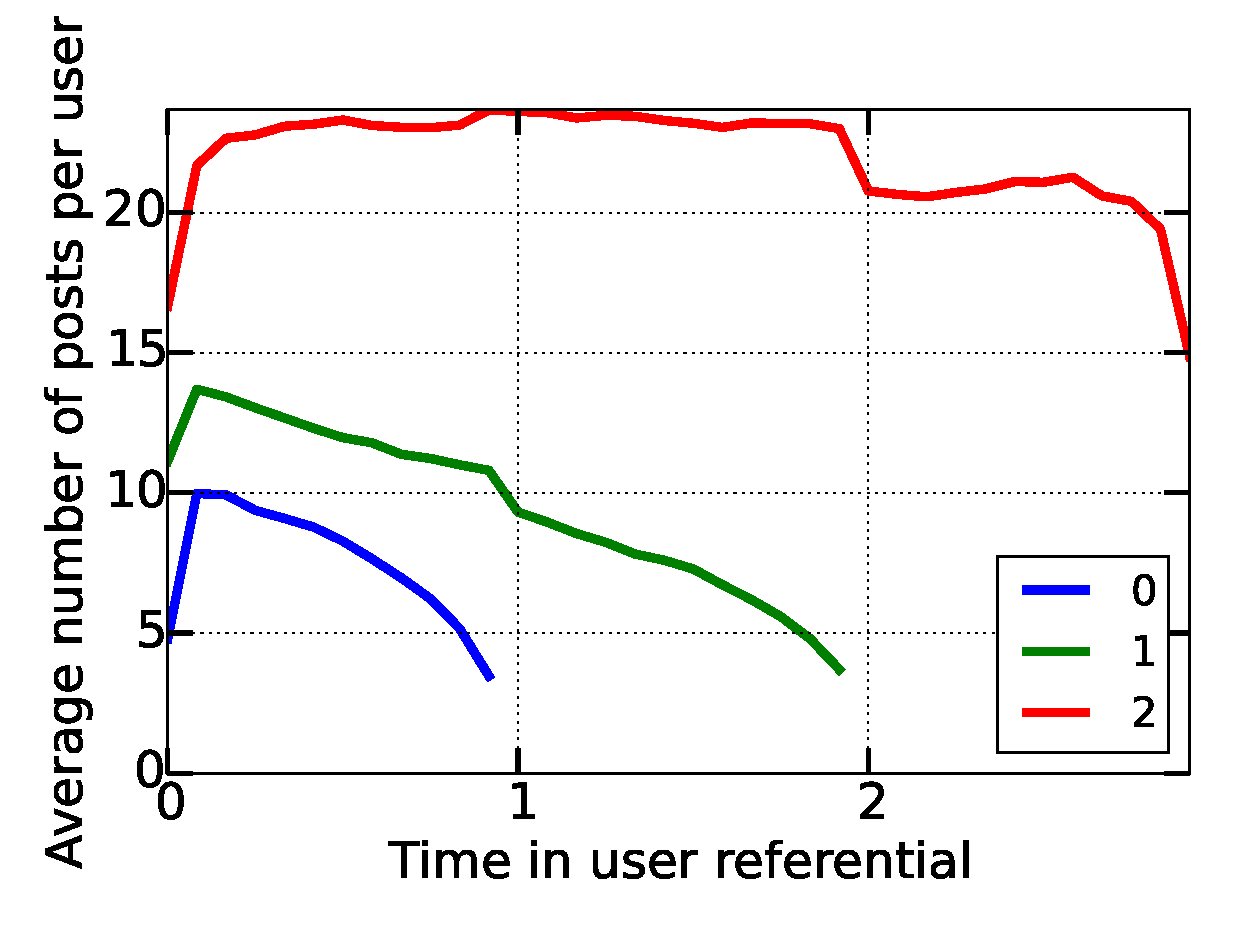
\includegraphics[scale=0.2]{./images/avr_posts_per_user_for_surviving_year_for_2012.eps}
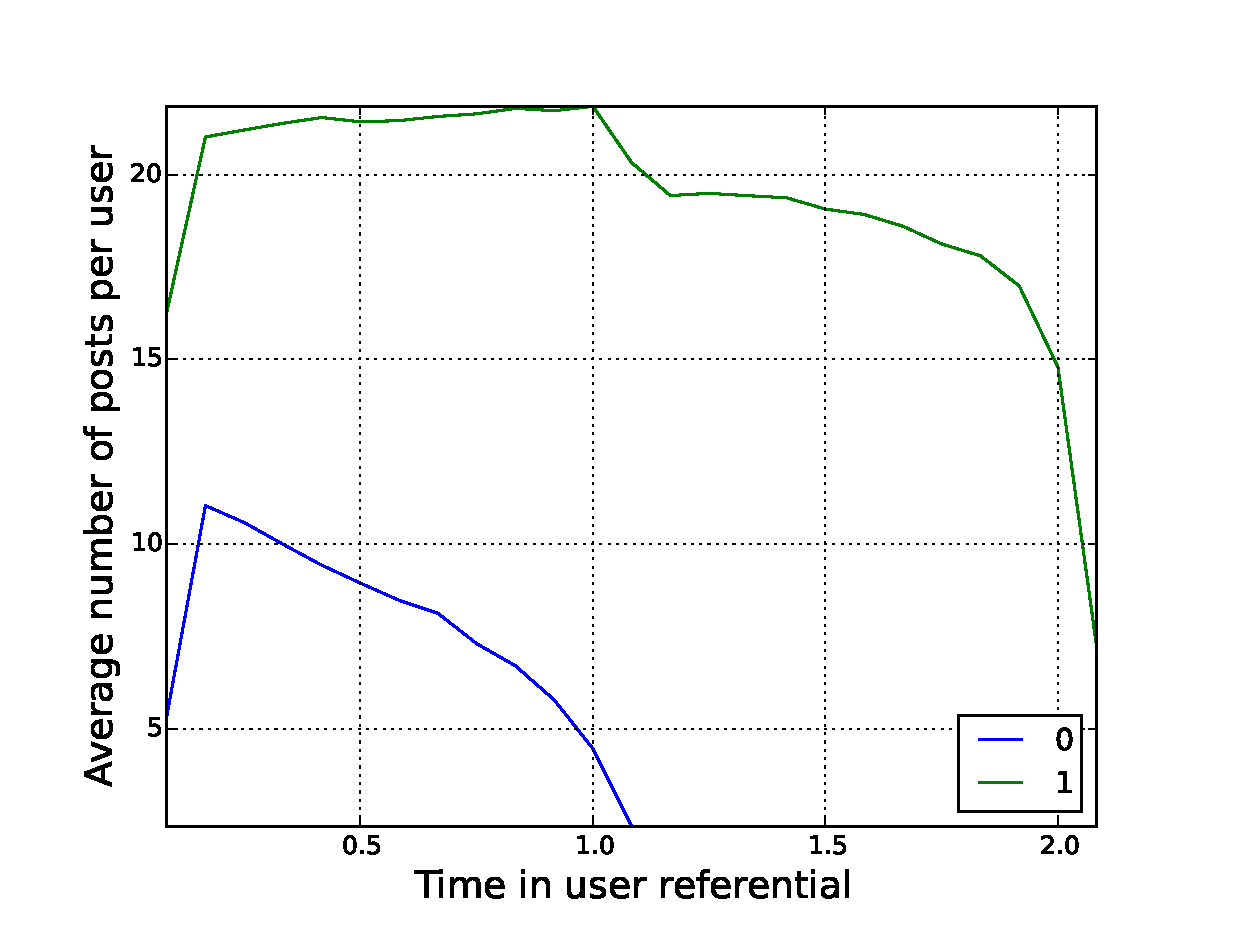
\includegraphics[scale=0.2]{./images/avr_posts_per_user_for_surviving_year_for_2013.eps}
\caption{Each figure corresponds to one cohort, from 2008 to 2013, left to right, top to bottom. The users for each cohort are further divided in groups based on how long they survived: users that survived up to 1 year are labeled 0, from 1 to 2 years are labeled 1, and so on. We observe that, for all cohorts, users that have a lower posting average are the first to die. We also observe that the posting  over time seem to decrease once we condition on the fact that users will survive a certain number of years. This suggests that the main reason for users to be posting less throughout the cohorts is because the mixture of users is different: there are more users that post less joining the network and the ones that post more are there to begin with, and they are the ones more likely to survive.}
\label{fig:avr_posts_per_user_for_surviving_year}
\end{figure}

Implicitly, the prior figure suggests that older (in the sense of first account activity) users are more active than newer ones, raising the question of whether newer users
are likely to eventually follow in older users' footsteps.  Analyzing users' behavior by cohort, grouping them by account creation year, is one reasonable way to address this question.  Figure~\ref{fig:avr_posts_per_user_over_time_cohorts} shows our first attempt at this analysis.  This figure already shows a significant cohort effect: users from latter cohorts appear to level off at a significantly lower posting average than users from earlier cohorts.  

However, the figure also has an awkward anomaly, the sharp increase in the average number of posts at the end of each cohort's first calendar year in Figure N.  Since we segmented our users by cohorts, by the end of each year onwards, we do not have users joining the network any more and the number of active users does not increase because of new users anymore. This fact, along with the observation that young users tend to post less from Figure~\ref{fig:NEEDED_avr_monthly_active_posts_relative}, drags the average down during the first year, since young users are always coming into the network.  
%% DC 10: A little redundant.  
% This is particularly true for the first month, specially considering that there are many user accounts that are created and only show activity for a single day in reddit, which likely brings the average down.

%% DC 10: I get tired of saying that; it would be useful to define "account creation" as the data handling part earlier as the first visible post in the dataset and just note that they actually created their account earlier than that.

We can largely account for this by still treating users as cohorts based on the year they first posted to reddit, but adjusting the time reference to be relative to the user's first post rather than clock time as we did before.  Figure~\ref{fig:avr_posts_per_user_cohorts_relative} presents this view of the data.

%% DC 10: Part of me would be curious about either an inset for the first three months, and/or a log-2 scale for time where the first year gets half the frame, etc.  My guess is that the log scale is hard to read because it's an unusual way to present time, but it does have an advantage in that most of the data is on the "left" of the graph and that would emphasize attention toward it, maybe.
This figure suggests that there may not be strong cohort effects early in a user's lifespan, although even after six months users in the most recent 2012 and 2013 cohorts appear to be less active than those in earlier groups.  In the long run, however, a striking pattern emerges: different cohorts stabilize in different levels of behavior, and in particular, the steady state activity for surviving users goes down for every year from 2008 to 2012.  

This raises interesting questions of why we see this behavior.  One plausible explanation is that users who find a community early in its life are also more likely than average to be those who will be attracted to it, in the same way that early ratings for a movie in a recommender system are likely to be higher than later ratings because the people who are most attuned to the movie are likely to see it earlier \cite{if_we_can_find_one}.  Another is an argument based on cumulative advantage, status, and attention-seeking: surviving users from earlier cohorts might be more capable of producing content that gets attention from other users.  This would lead to them getting more comments and votes for their content, and people who get positive attention are more likely to return \cite{joyce-kraut, wikipedia, everything2_papers}.  

We're not taking a position on either of these as the mechanism that explains these results; both would be interesting avenues for future work.  We do suggest that looking at Reddit from a cohort and user-based view rather than an aggregate community view helped us uncover interesting phenomena and questions that would have been invisible to more commonly-performed analyses of community behavior. 

%% DC 10: The status bit is intriguing but needs to be explained a little better.  Took a little shot at it but framing it in terms of cumulative advantage rather than status
%% DC 10:This, too, would need to be explained/justified/supported, and I can't come up with a plausible one, so deleting it.
%Yet another explanation would be that earlier users demographics were different in terms of age and interests, for example, and these correlate to the fact that they present a higher activity.

%% DC 10: There is a mysterious question about why 2008 ramps up more slowly, that I would interpret in the "there was less to comment on" framing that we've chatted about before.  You could actually do an analysis to test this, where for each user, the number of posts in a month is normalized by the number of posts made in reddit in that month: that is, how active is the user relative to the total amount of activity in reddit.  This is _not_ a linear scaling when the analysis is relative to the user's initial start date, and I would be curious to see what it showed.


%%%% DanCo stopping here %%%%

%% DC 10: These are actually a separate section, or sections, for me.  In particular, Users' Effort and the Simpson almost certainly need to be combined.  

\subsection{Effort per Comment}

In addition to the raw number of posts, comments length can also be considered as a proxy for user effort in the network. Users that type more put more of their time in the network, contribute with more content and might create stronger ties with the community. The Figure N shows the evolution of the monthly average comment length in reddit.

\begin{figure}[!tb]
\centering
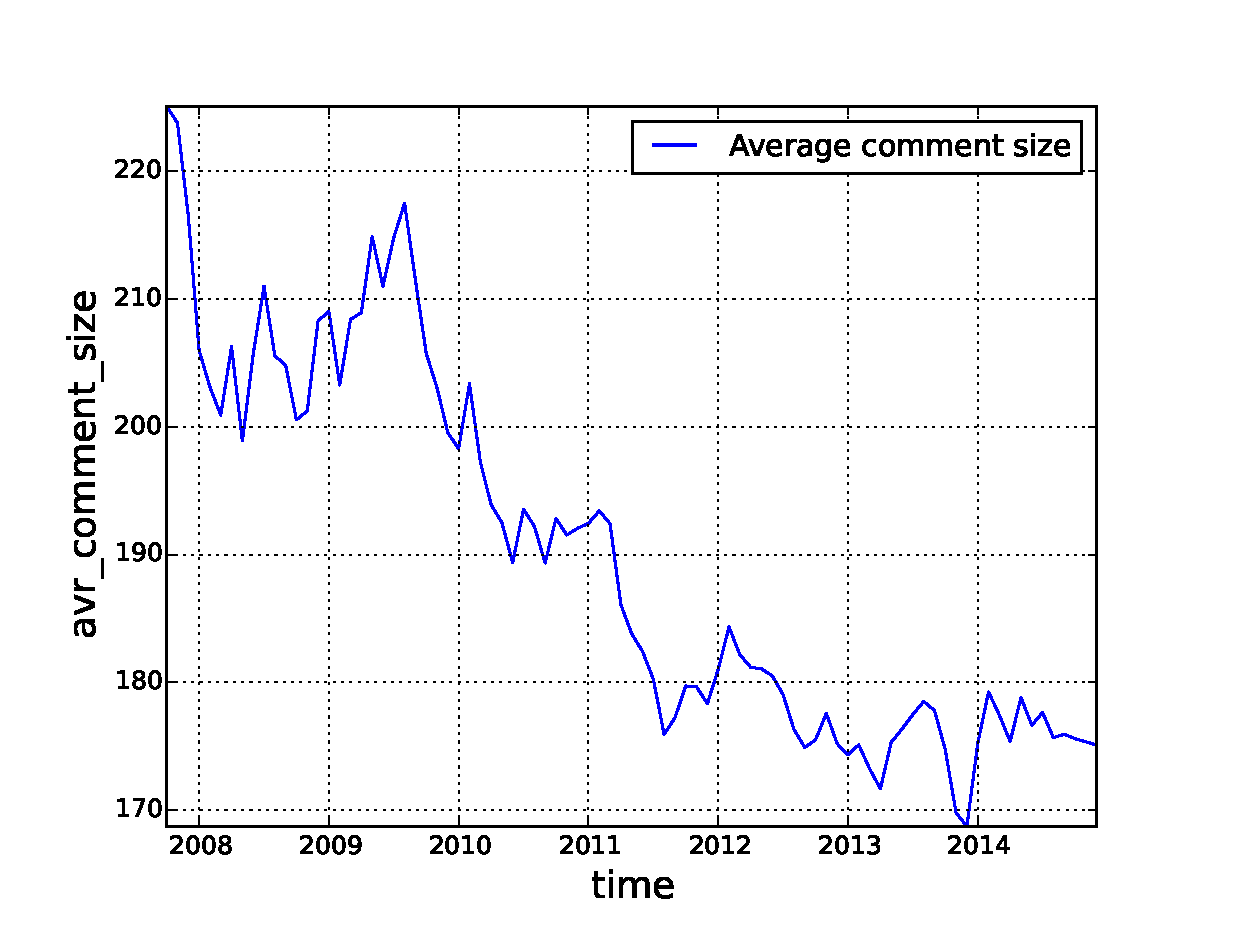
\includegraphics[scale=0.4]{./images/avr_comment_size_over_time_total.eps}
\caption{Average comment size (number of characters) over time for the reddit network. We observe that there is a decreasing trend for the average comment size. This means that users, on average, are making smaller comments in reddit as time passes. This, however, hides important aspects of user behavior over time and does not mean that users, as they survive in the network, write smaller comments.}
\label{fig:avr_comment_size_over_time_total}
\end{figure}

\begin{figure}[!tb]
\centering
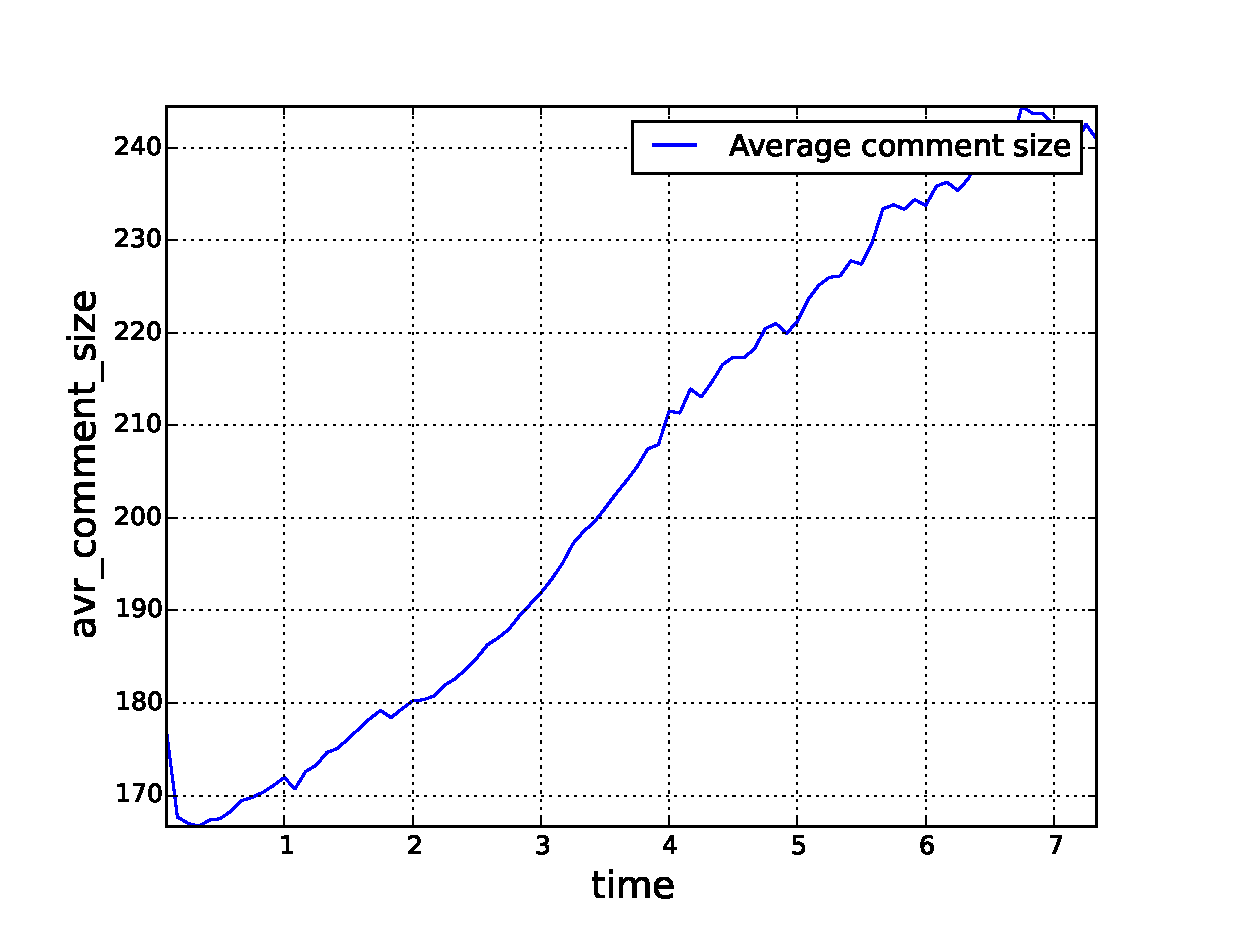
\includegraphics[scale=0.4]{./images/avr_comment_size_user_ref_total.eps}
\caption{Average comment size from the users time referential. This shows that comment length made by users increase for users that lived longer in the network, save for a small decrease in the initial time. This, however, is also not enough to say that we should expect the average size of the comments in the network to increase since the users that survive write longer comments.}
\label{fig:avr_comment_size_user_ref_total}
\end{figure}

Based on the downwards tendency of the comment length, one could possibly imagine that the user commitment with the network is lowering over time. This, however, might not be the best way to interpret this information. Figure N shows the comment length per cohort based on the user referential time. This figure shows that, unlike the average overall network comment length, surviving users increase the size of their contributions to the community over time. This is true for all users cohorts. The important thing to notice here is that, while user comments get longer as they stay for longer in the network, younger users start from a lower baseline comment than older users. Together with the fact that recent reddit has experienced exponential-like growth, the heavier weight when evaluating the averages for Figure N as the years go by is shifted towards the size of the ever growing younger generation, and this younger generation brings the average down since they start writing less.

Some possible explanations for this difference in the starting points could be that older users are, again, sampled from a different demographics that is more committed and willing to spend more effort into developing their virtual identity. Also, it could be that it is a natural evolution of the community, as older users have taken most of the main space of interests when it comes to creating new subreddits and starting these communities, new users have it all already made and sometimes might feel intimidated or not motivated to create new topics or communities that already exist or that are less likely to compete with the existing ones. In a way, these new users could behave more as lurkers, while the older users are the ones that laid the foundation of reddit.

\begin{figure}[!tb]
\centering
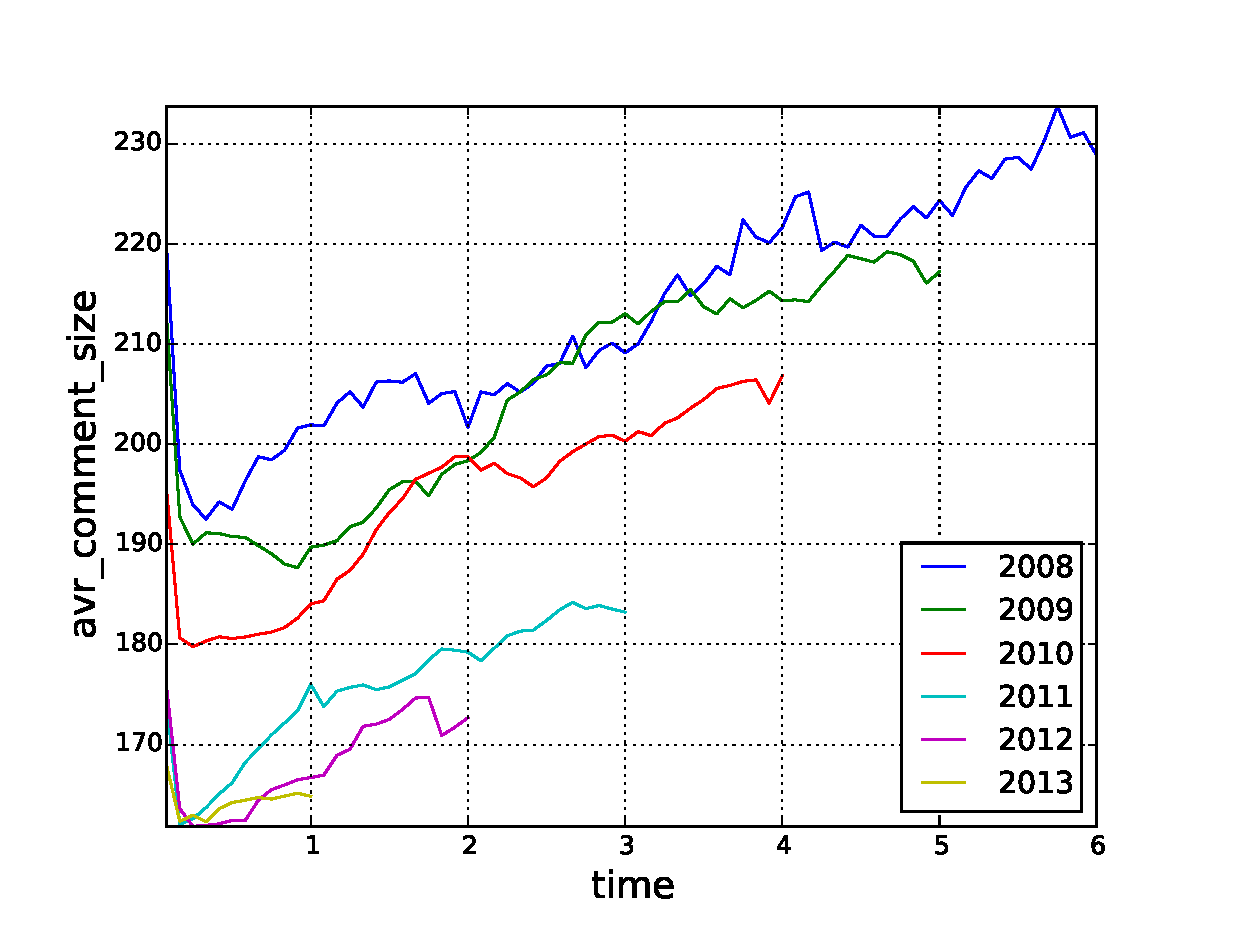
\includegraphics[scale=0.4]{./images/avr_comment_size_cohorts.eps}
\caption{Average length of comments from the user time referential segmented by user creation cohorts. This figure start to explain why we see different trends in the overall network comment length and user referential overall comment length. It shows that, as users come from latter cohorts, they start from a lower commenting length average compared the the earlier cohorts. This, together with the fact that reddit is growing exponentially in terms of users means that \textit{we have an influx of users that make smaller comments than the previous generations}, although even for them, as they survive, they make longer comments. Just as for the users' posting average, we can not distinguish based on this graphic alone whether users that make smaller comments leave the network earlier or they indeed write longer comments as they survive. Figure \ref{fig:avr_comment_length_for_surviving_year} sheds some light on this question.}
\label{fig:fig_label}
\end{figure}

\begin{figure}[!tb]
\centering
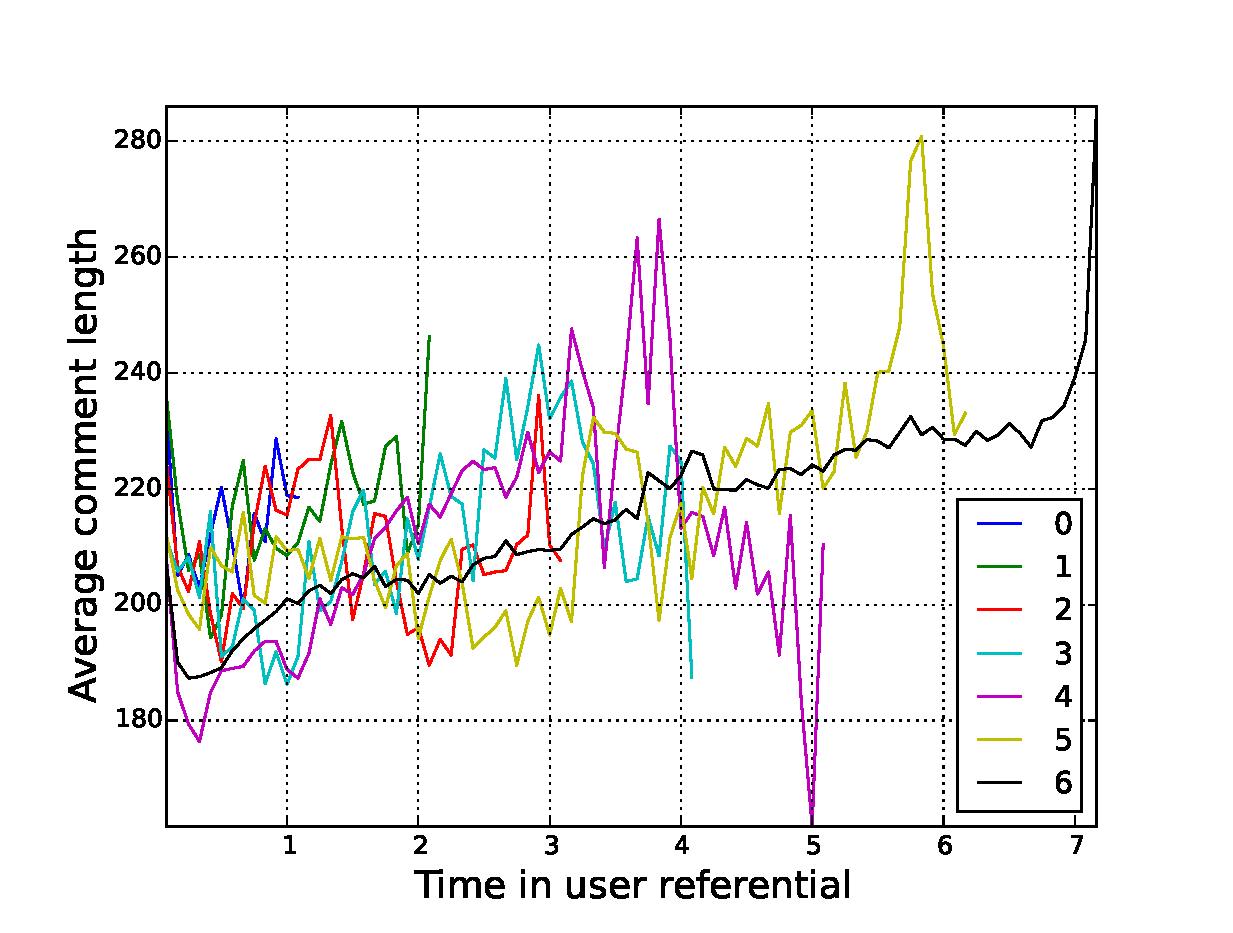
\includegraphics[scale=0.2]{./images/avr_comment_length_for_surviving_year_for_2008.eps}
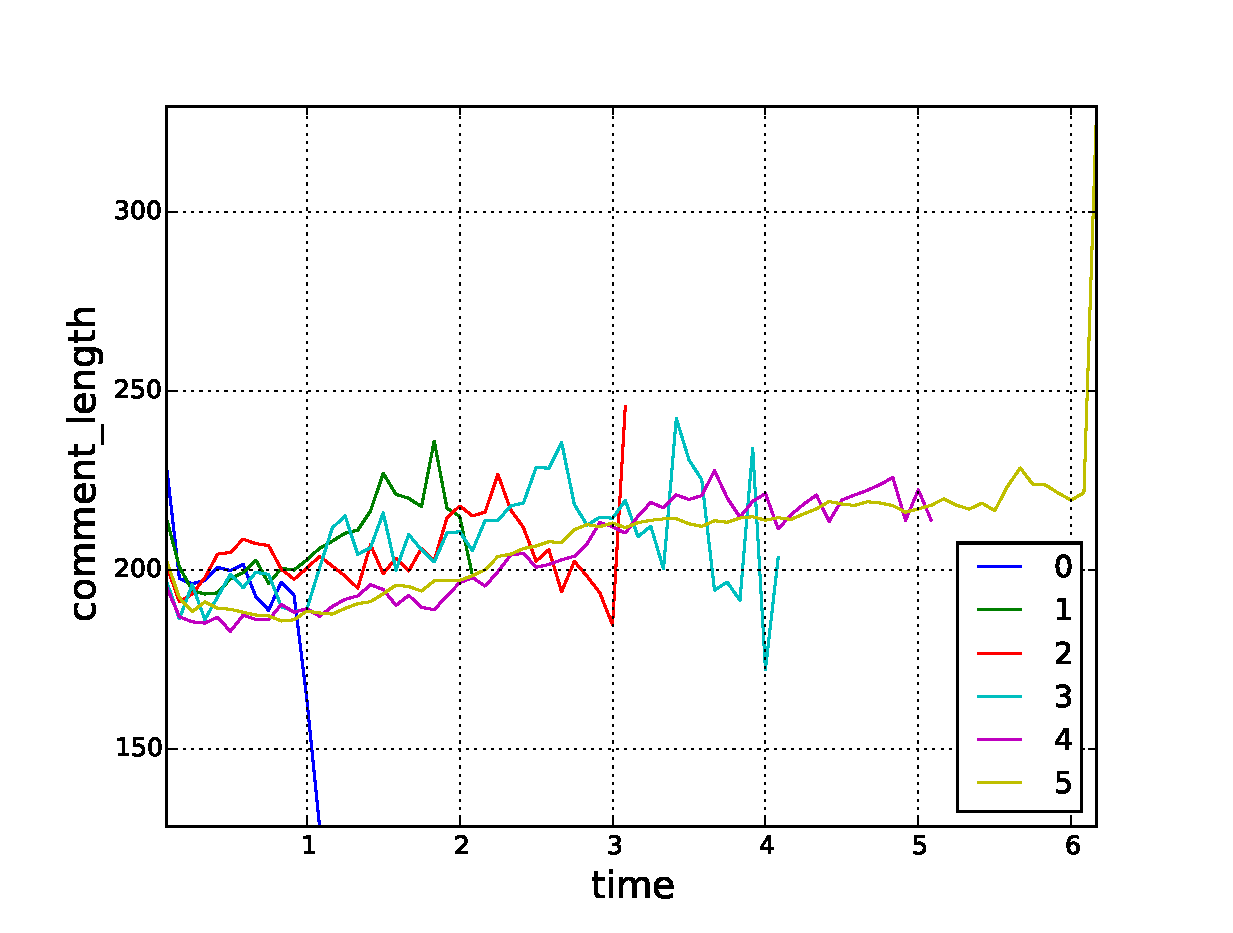
\includegraphics[scale=0.2]{./images/avr_comment_length_for_surviving_year_for_2009.eps}
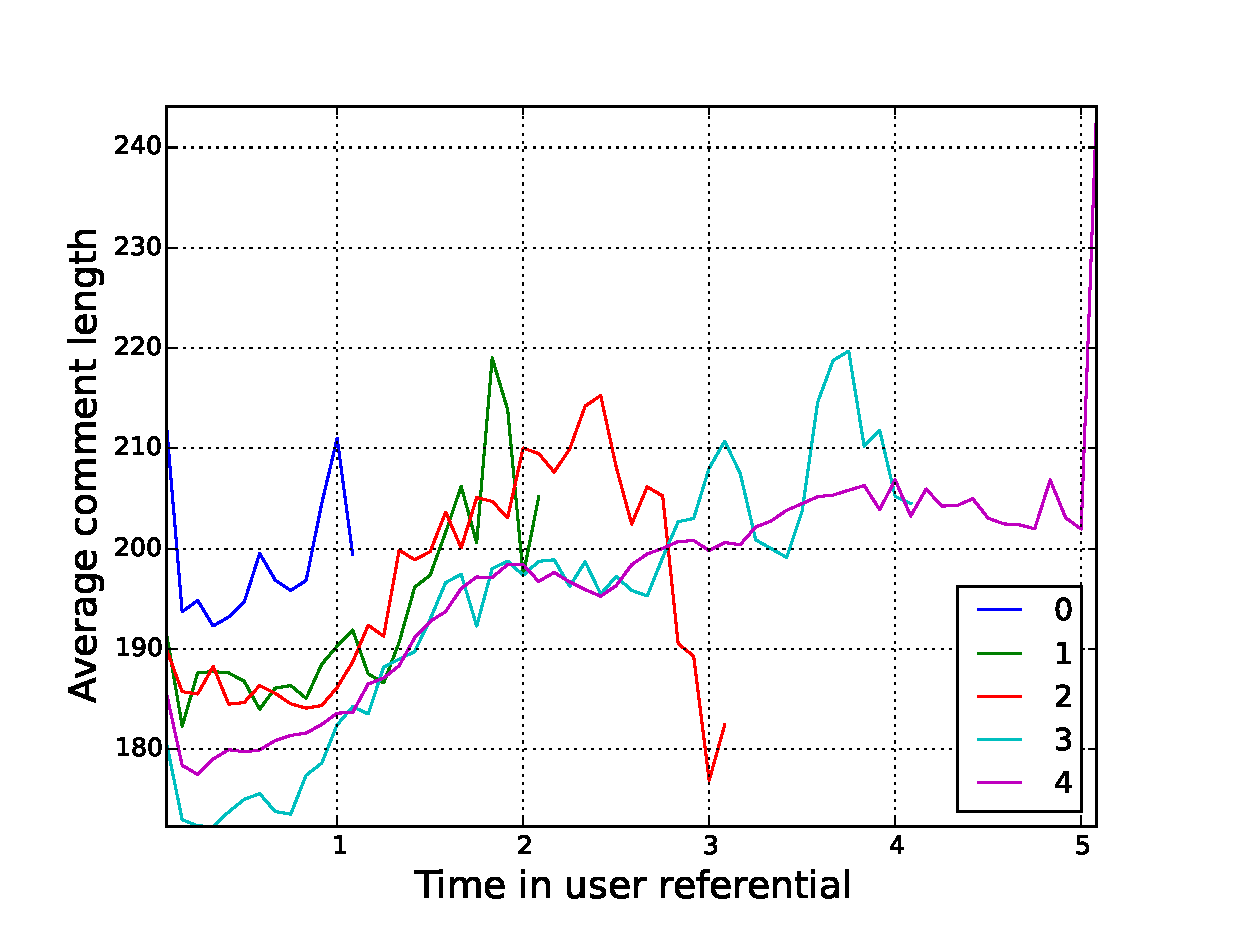
\includegraphics[scale=0.2]{./images/avr_comment_length_for_surviving_year_for_2010.eps}
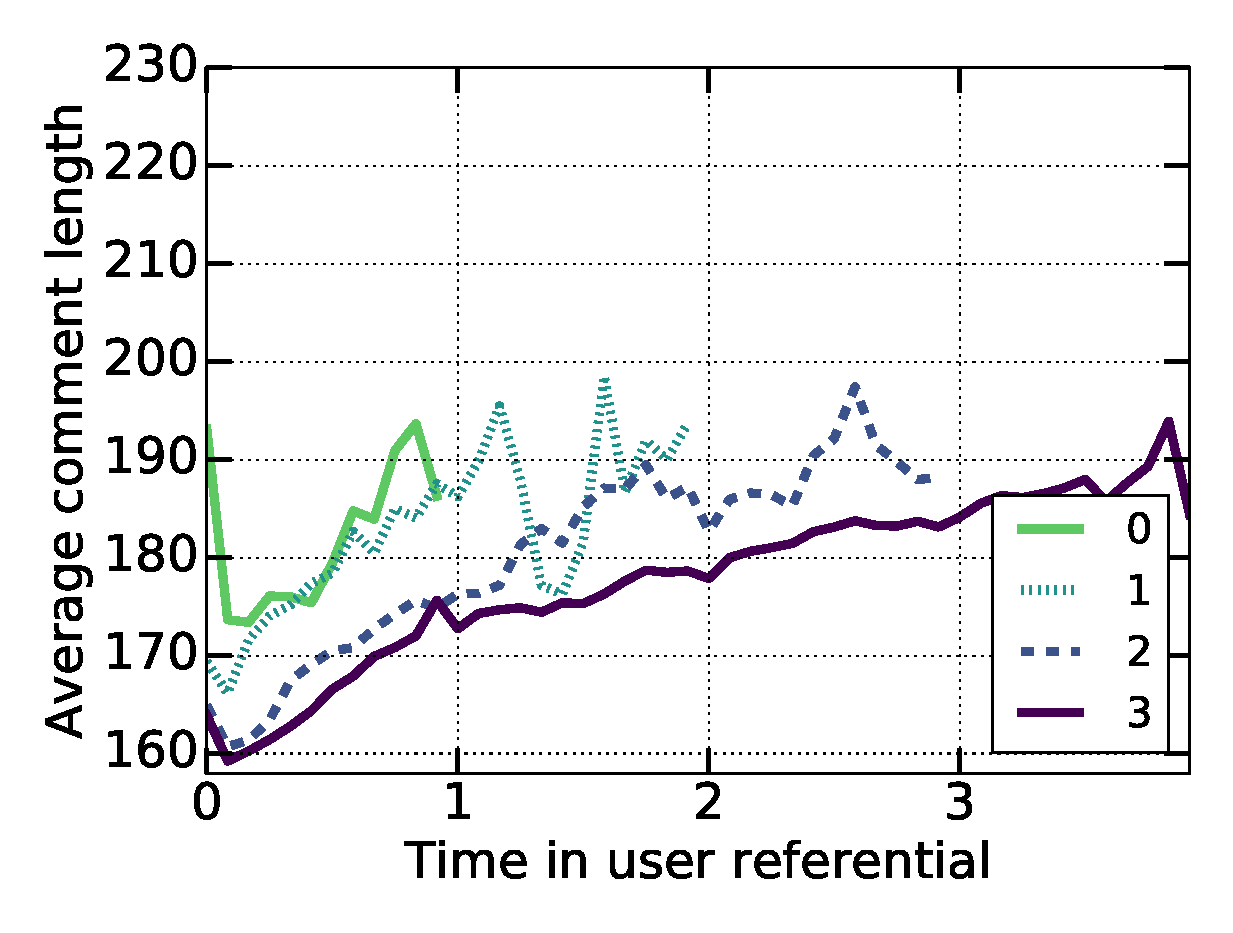
\includegraphics[scale=0.2]{./images/avr_comment_length_for_surviving_year_for_2011.eps}
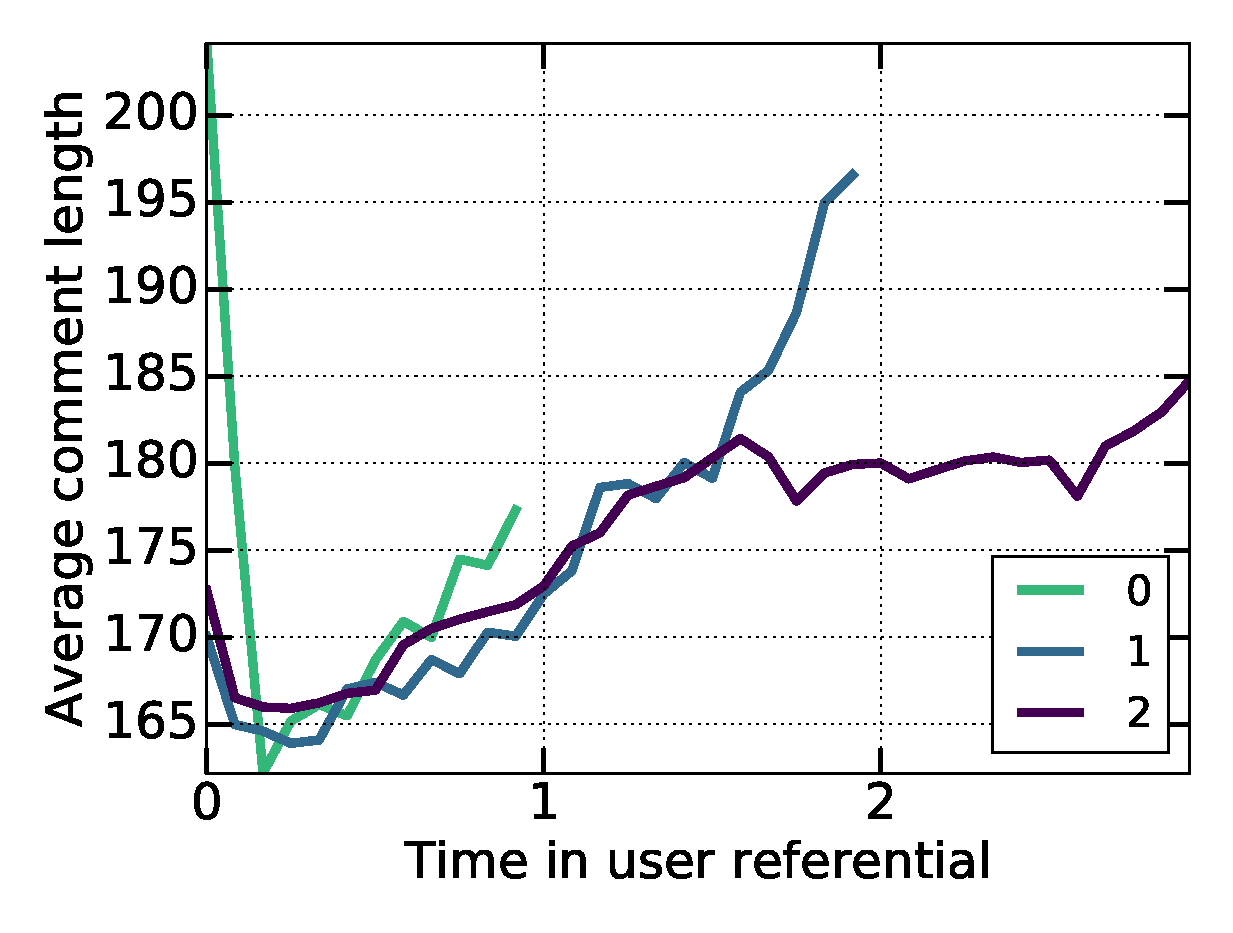
\includegraphics[scale=0.2]{./images/avr_comment_length_for_surviving_year_for_2012.eps}
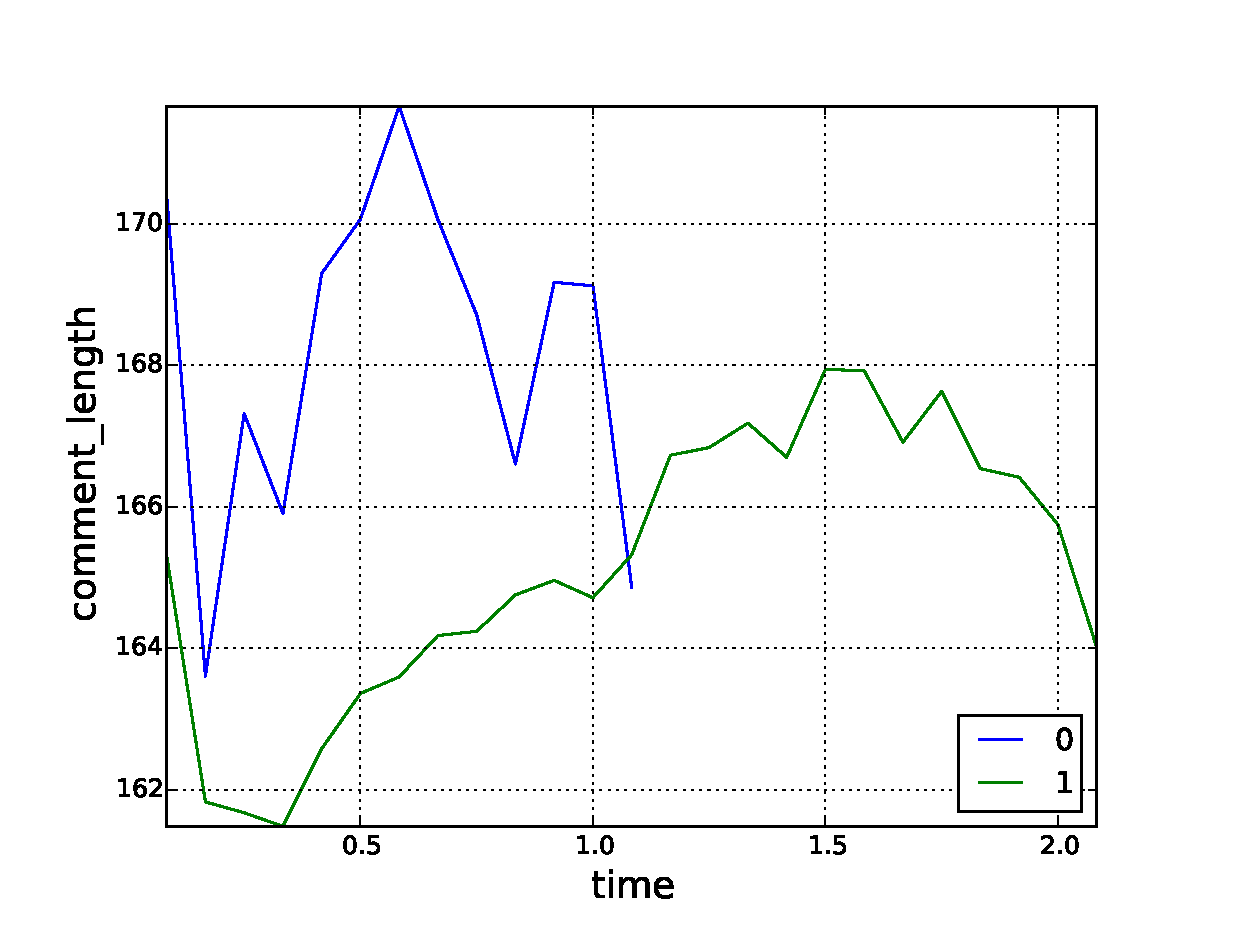
\includegraphics[scale=0.2]{./images/avr_comment_length_for_surviving_year_for_2013.eps}
\caption{Just as in Figure \ref{fig:avr_posts_per_user_for_surviving_year}, each figure corresponds to one cohort. These figures show the average comment length for users segmented by the number of years that he/she survived in the network, given a cohort. Here, we make two important observations: first, \textit{comment length do increase inside of each cohort}, no matter how long the user survives. Secondly, as a general trend, \textit{users that make longer comments inside of each cohort die faster}. This is quite surprising, given that we would expect people to put less effort when they are more likely to stop using the network.}
\label{fig:avr_comment_length_for_surviving_year}
\end{figure}

Yet another hypothesis that we might consider is that users are lowering their activity due to an ``initial value problem''. We can imagine that users, as they join the network, they tend to produce content according to the norms of what they see. If we look at the cohort posting size over time superimposed with the average size for the whole network, we can see that the starting point of each cohort seems to agree to a reasonable extent to the average over the total network. This way, users would be simply reproducing things as they see in their early months, but as we have seen in Figure N, users start their life posting longer content, but there is a strong decrease in size for the early months before the size increases for the surviving users.

\begin{figure}[!tb]
\centering
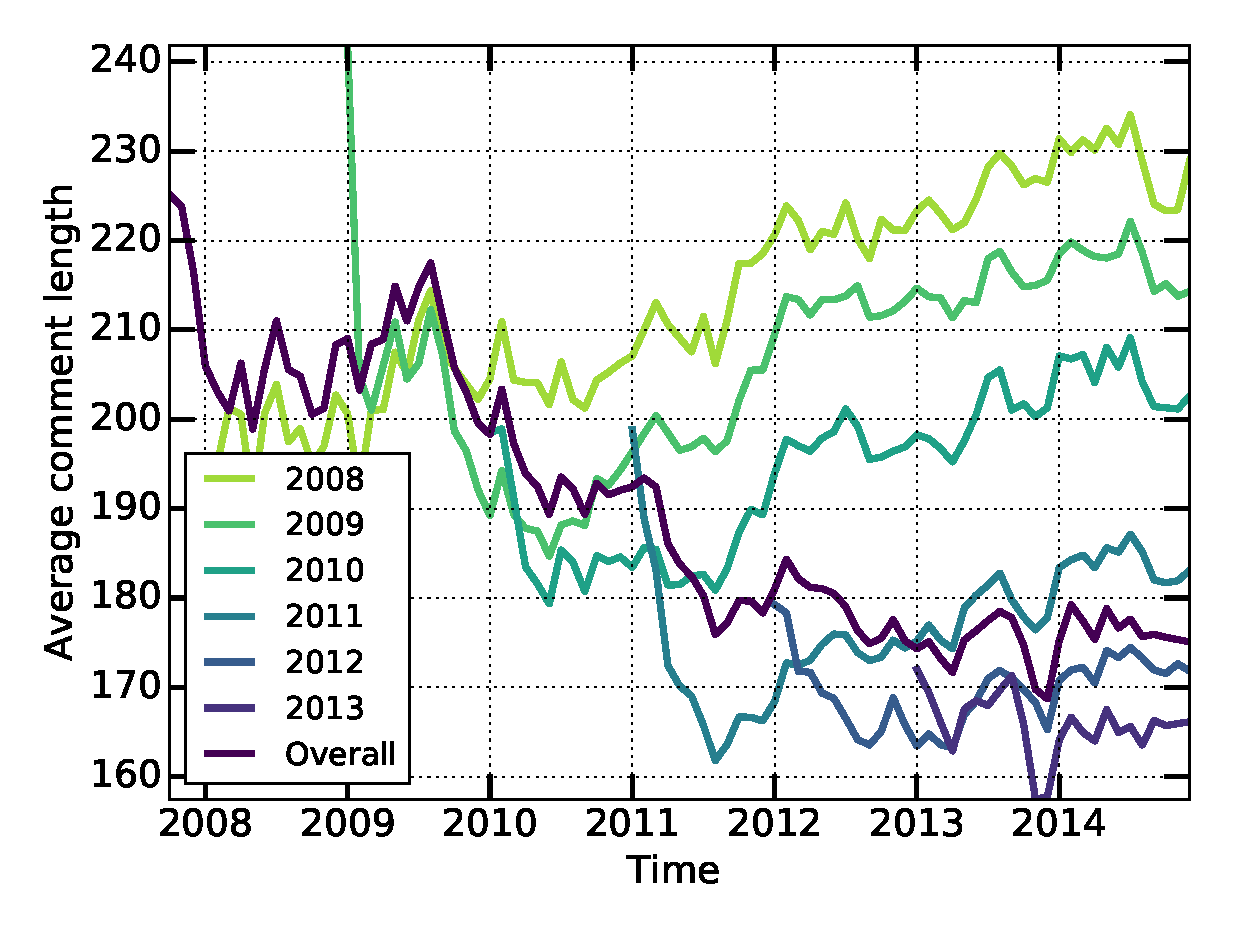
\includegraphics[scale=0.4]{./images/avr_comment_size_over_time_cohorts.eps}
\caption{Average comment length over time for cohorts on user creation time superimposed over the trend for the total of users. Here we observe how the early existence for each cohort has a reasonable agreement with the overall trend. This might indicate how the new users might be just adopting the community norms regarding comment length.}
\label{fig:fig_label}
\end{figure}

\subsection{Activity Nature}

One common question from the literature is what sorts of activities users engage in; this can be used as a metric of community health (cites) or to categorize users into roles they play in the community (cite).  In reddit, we do not have per-user voting behavior, but we do have the number of comments and submissions, and a naive view of this would look at the ratio of comments to submissions over time.

While submissions can be considered new content that an author generates, a comment can be considered as a contribution to an existing content from another author. Since the total number of comments always surpasses the number of submissions, Figure N shows the evolution of the ratio of comments per submission over time for users created from 2008 until 2013. It is important to highlight here that we are not talking about the average number of comments a submission gets, but how many comments a user authors for each of his/her submissions.

%% Sam 10: It just occurred to me that although the comment size is decreasing, users might be putting just the same amount of effort, just writing more comments. This figure that shows that the newer cohorts comment more might mean that users are actually typing the same amount, but they are pulverizing more their efforts. Might be worth to comment about it, although it obviously raises the question of why we didn't do it. I can try to generate this results on monday, it is likely easy to do so.
%% Sam 10: Thinking again about it, I raise the question of weather users are getting ``lazier'' many times in the text. This should be included. Can probably make up for the removal of the subreddits section due to the fact that we have a lot of default 2008 subreddits.
\begin{figure}[!tb]
\centering
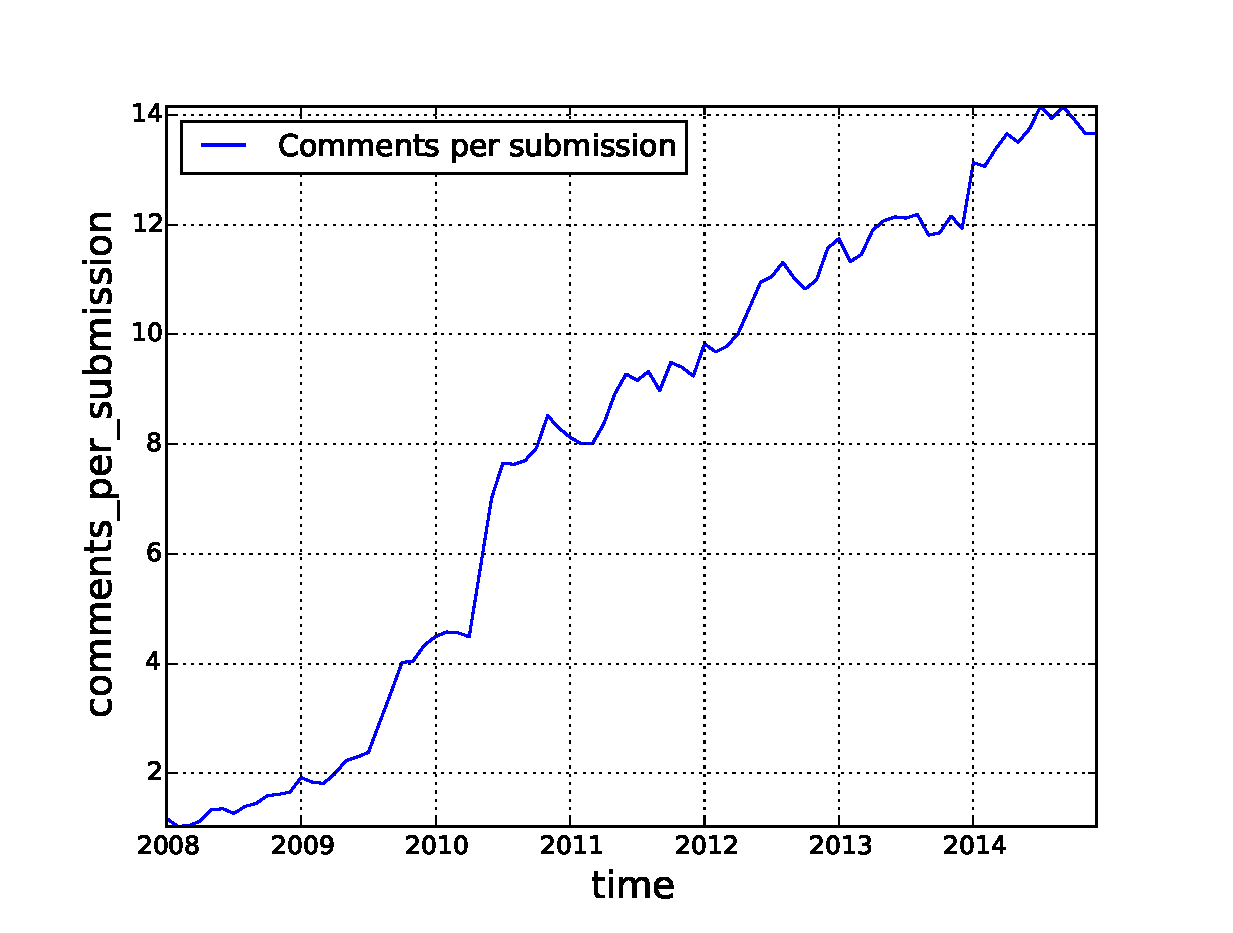
\includegraphics[scale=0.4]{./images/comments_per_submissions_over_time_total.eps}
\caption{Comments per submission ratio for reddit over time. We observe an overall increasing trend of comments for each submission. Notice that these should not be interpreted as how many comments each submission gets, but as how many comments users author for each submission --- submissions might get comments a long time after they are posted, by users from different years. This distinction becomes more important when we change the time referential and separate users by cohorts.}
\label{fig:comments_per_submissions_over_time_total}
\end{figure}

\begin{figure}[!tb]
\centering
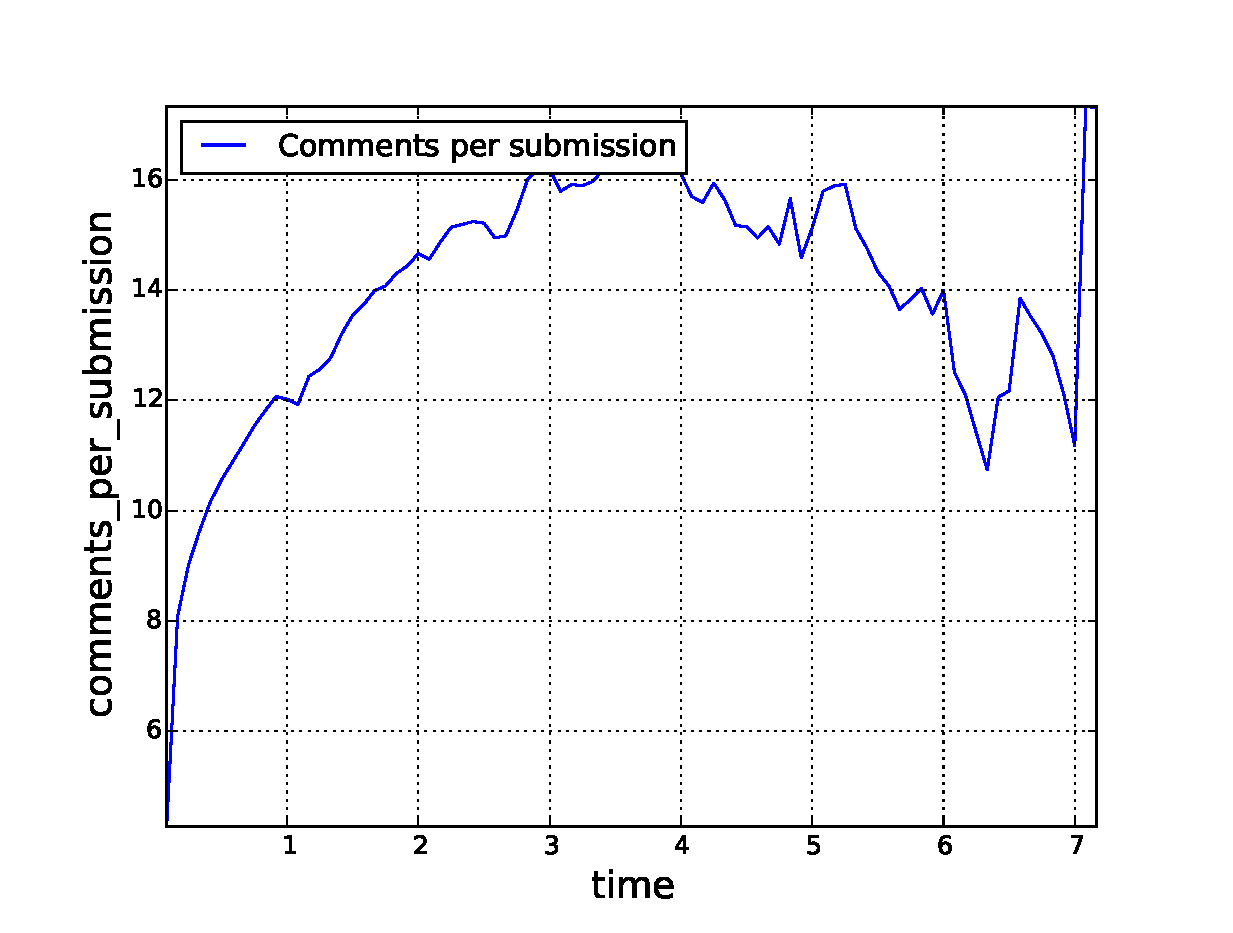
\includegraphics[scale=0.4]{./images/comments_per_submissions_user_ref_total.eps}
\caption{Comments per submissions ratio from the user referential. This should be interpreted as how many comments a user makes for each submission in their x-th year of existence. We observe an interesting overall trend that peaks between 3 and 4 years of existence. This, however, does not mean that users will necessarily decrease their behavior as they live longer, but that given that a user has survived for x years, what is his/her comment per submission ratio likely to be.}
\label{fig:comments_per_submissions_user_ref_total}
\end{figure}

We have found that segmenting users and subreddits by cohorts on the years that of the first comment highlights significant differences of behavior and help us to understand how reddit changed over these years.


Table 1: Number of distinct users that authored comments and submissions segmented by the year of the first post of the user. The Total numbers are based on posting data from 2007 until 2014, corresponding to our full dataset. The Oct 1st, 2014 onwards numbers are based on the last 3 months of data we have, and we consider this as the current, active reddit.


Table 2: Number of distinct subreddits segmented by the year of the first post of the user. The Total numbers are based on posting data from 2007 until 2014, corresponding to our full dataset. The Oct 1st, 2014 onwards numbers are based on the last 3 months of data we have, and we consider this as the current, active reddit.

Table indicates that reddit grew significantly from 2007 until 2012, practically doubling the number of new users per year for each of these years, with similarly significant growth in subreddits. Although the most expansive growth happened in the first years, more than half of the registered users are from the last 2 years, and their behavior is significantly different than previous users, impacting in the overall behavior of the community. For instance, users from the 2014 cohort have a higher tendency to make submissions instead of comments, in contrast with all the previous cohorts.

Looking at the user time referential, the evolution of the number of comments per submission shows a decreasing trend for the older cohorts. One explanation for this is that, as the community grew, more content from an absolute point of view was present in the social network, and therefore users had more reason to make contributions commenting instead of submitting new content that was likely to already exist.

%% DC 10: This needs to be managed better, somehow; right now it's a little overwhelming as a blob of graphs.  It might be better to pick one representative year rather than present them all.  Also, this might an excellent place to introduce (or reintroduce) the point that when you zero-adjust, you have less and less data off to the right; the abrupt jumps that especially the later years (4, 5, 6) from the earlier cohorts show at the end are almost surely driven by low n users, right?
\begin{figure}[!tb]
\centering
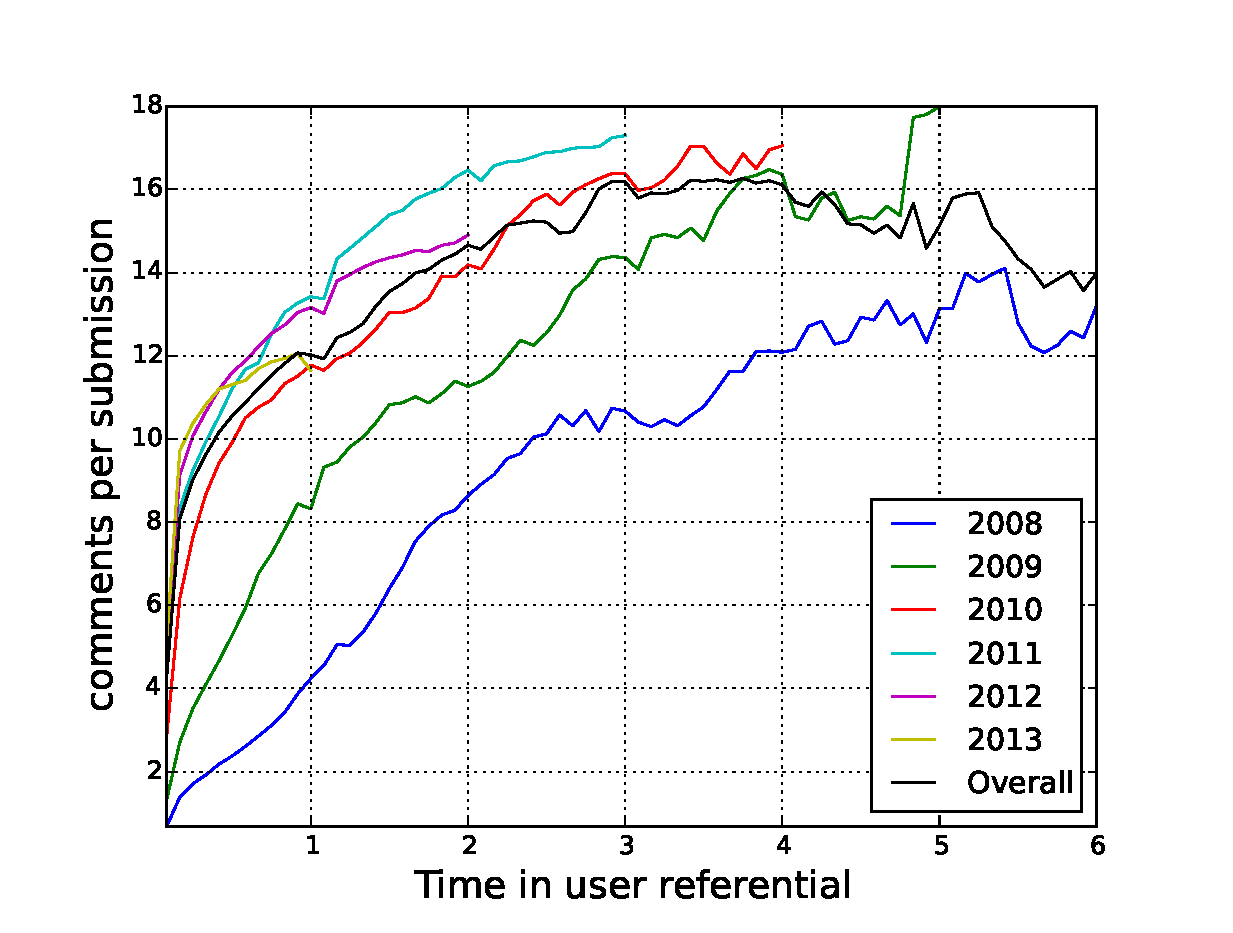
\includegraphics[scale=0.4]{./images/comments_per_submissions_cohorts.eps}
\caption{Comments per submissions cohorted by user creation year. Here we observe that, unlike the total aggregated graphic, all users are are increasing the number of comments per submissions, but latter cohorts show a much higher level of comments per submissions than earlier cohorts. This brings the initial part of the aggregated user-referential curve up, while the end of the curve consists only of users from the latter cohorts that preset an lower ratio. It is also important to notice that, as these curves move to the right, less comments and submissions exist in the bins, for there are less users that survived for such long periods. This results in some spiky behavior in the rightmost end of some curves due to the reduced amount of data. Just as with the previous user-referential cohort curves, we can not distinguish solely based on this graphic if users are increasing their commenting behavior or if the users that do not comment die earlier. Figure \ref{fig:comments_per_submissions_for_surviving_year} help us to answer this question.}
\label{fig:comments_per_submissions_cohorts}
\end{figure}

\begin{figure}[!tb]
\centering
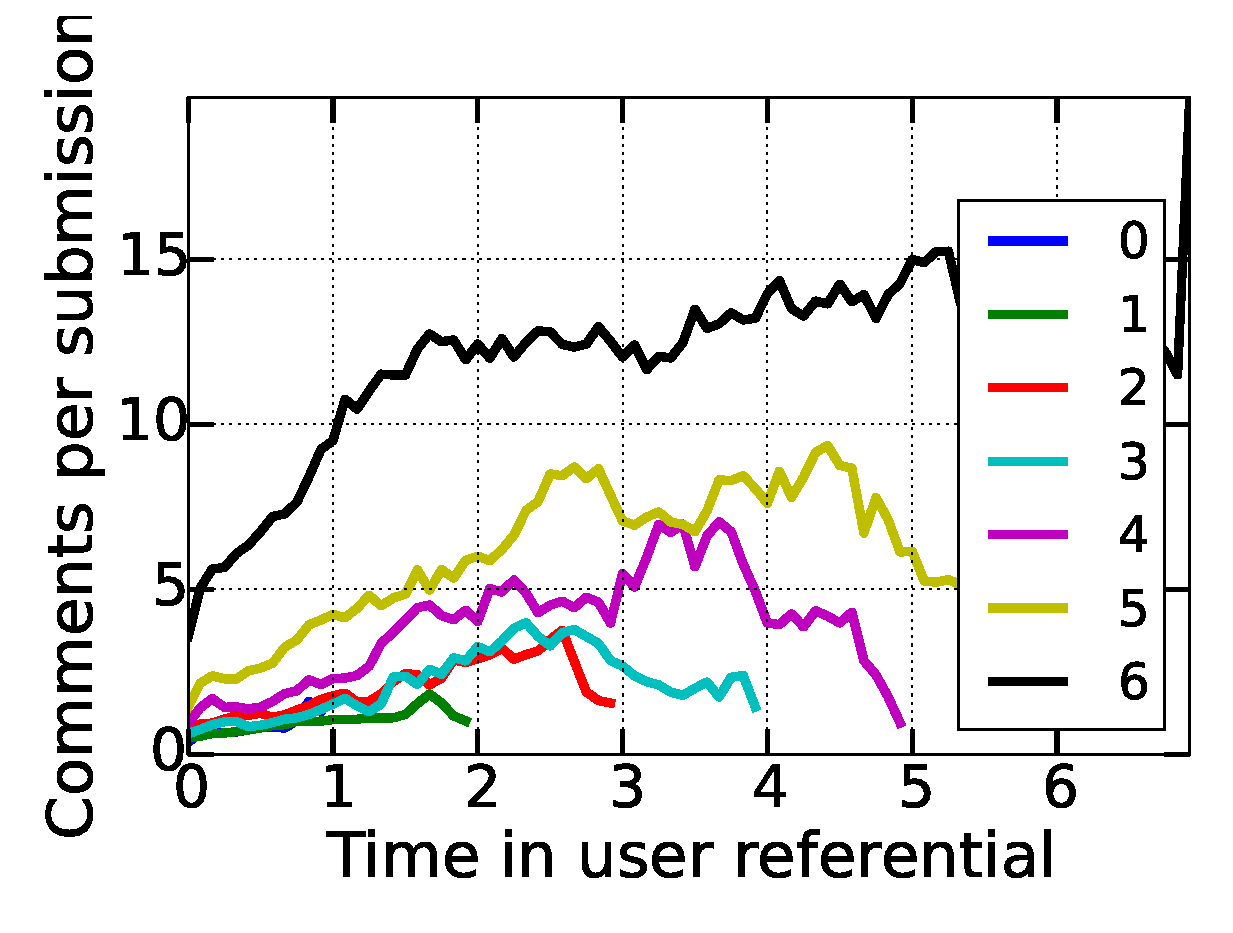
\includegraphics[scale=0.2]{./images/comments_per_submissions_for_surviving_year_for_2008.eps}
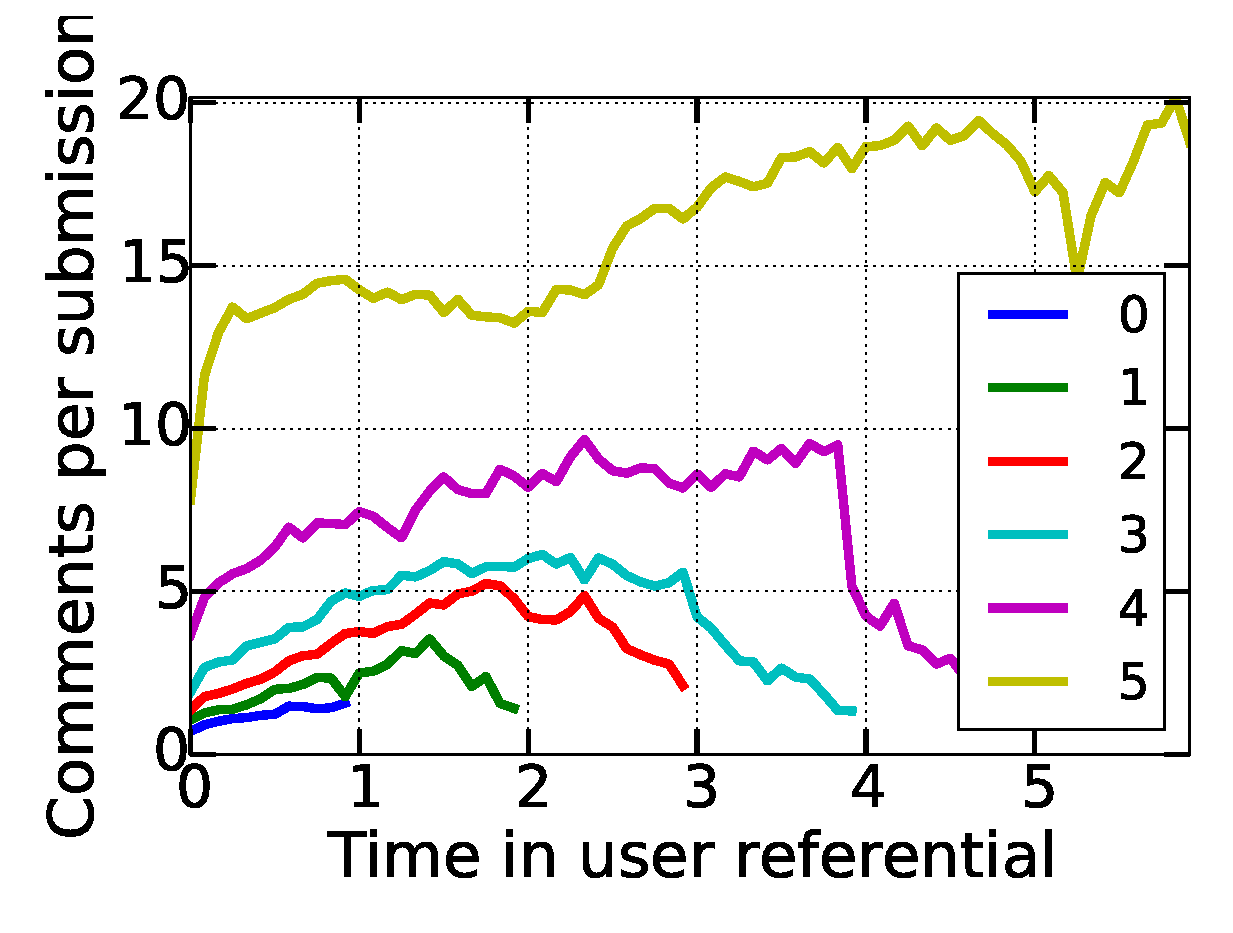
\includegraphics[scale=0.2]{./images/comments_per_submissions_for_surviving_year_for_2009.eps}
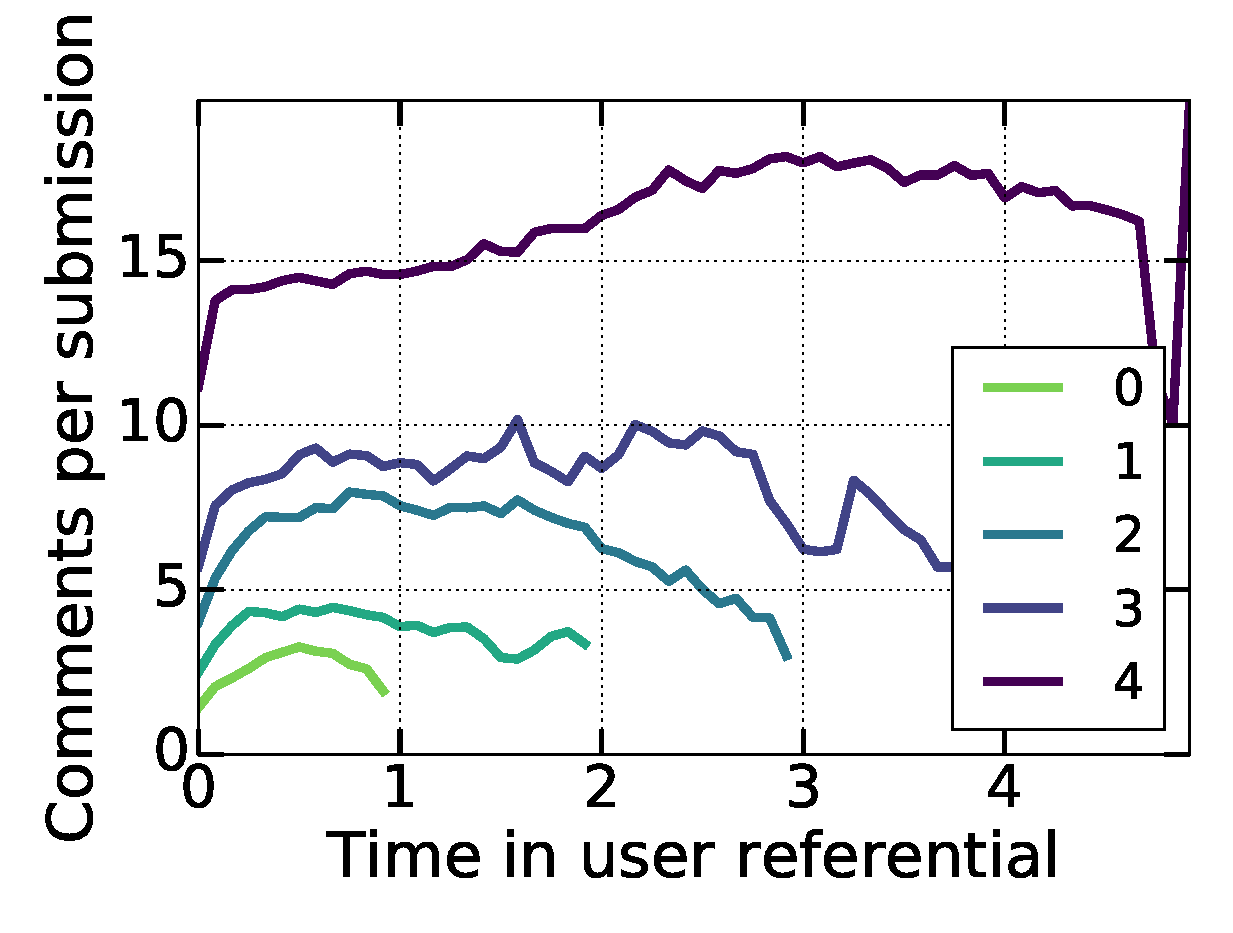
\includegraphics[scale=0.2]{./images/comments_per_submissions_for_surviving_year_for_2010.eps}
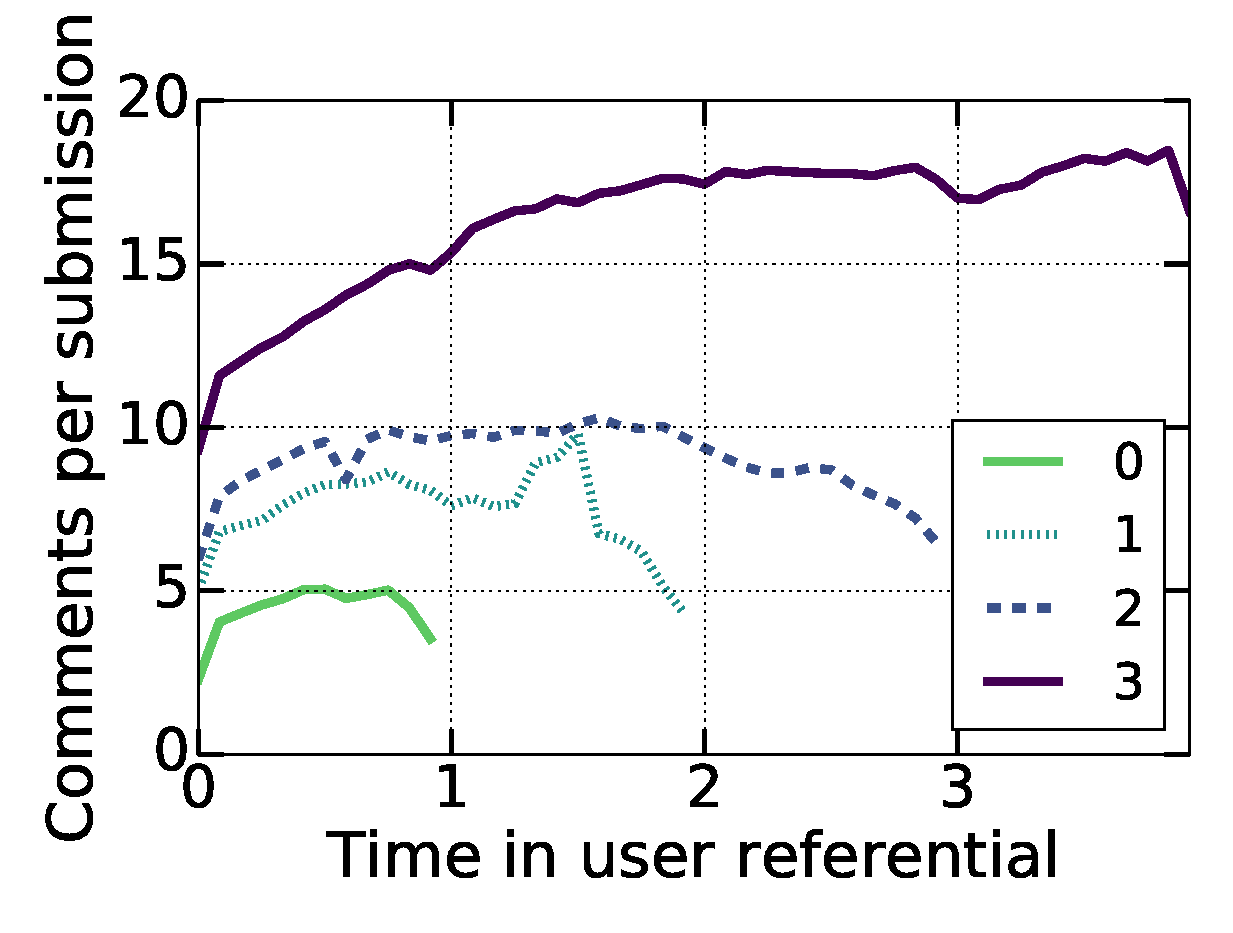
\includegraphics[scale=0.2]{./images/comments_per_submissions_for_surviving_year_for_2011.eps}
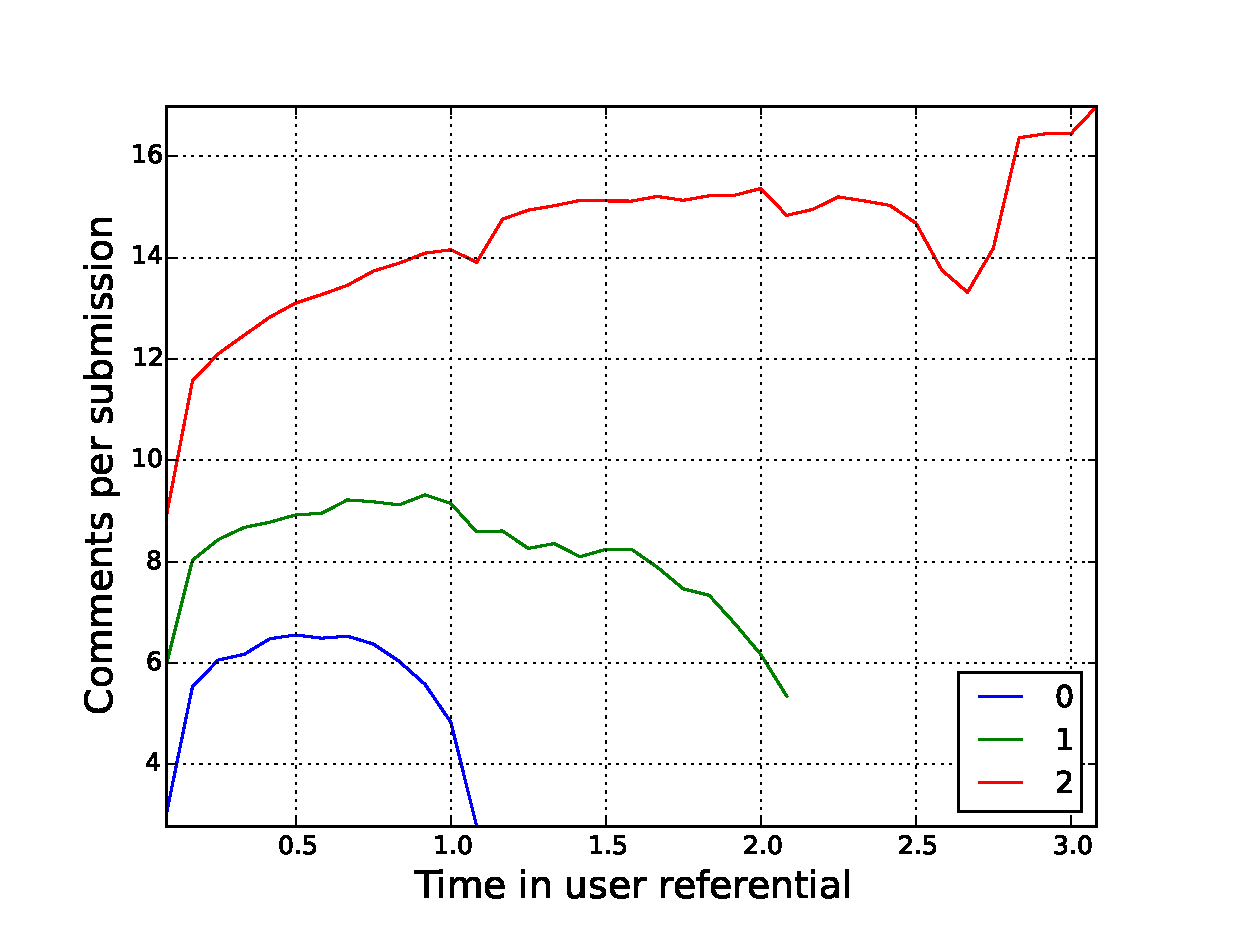
\includegraphics[scale=0.2]{./images/comments_per_submissions_for_surviving_year_for_2012.eps}
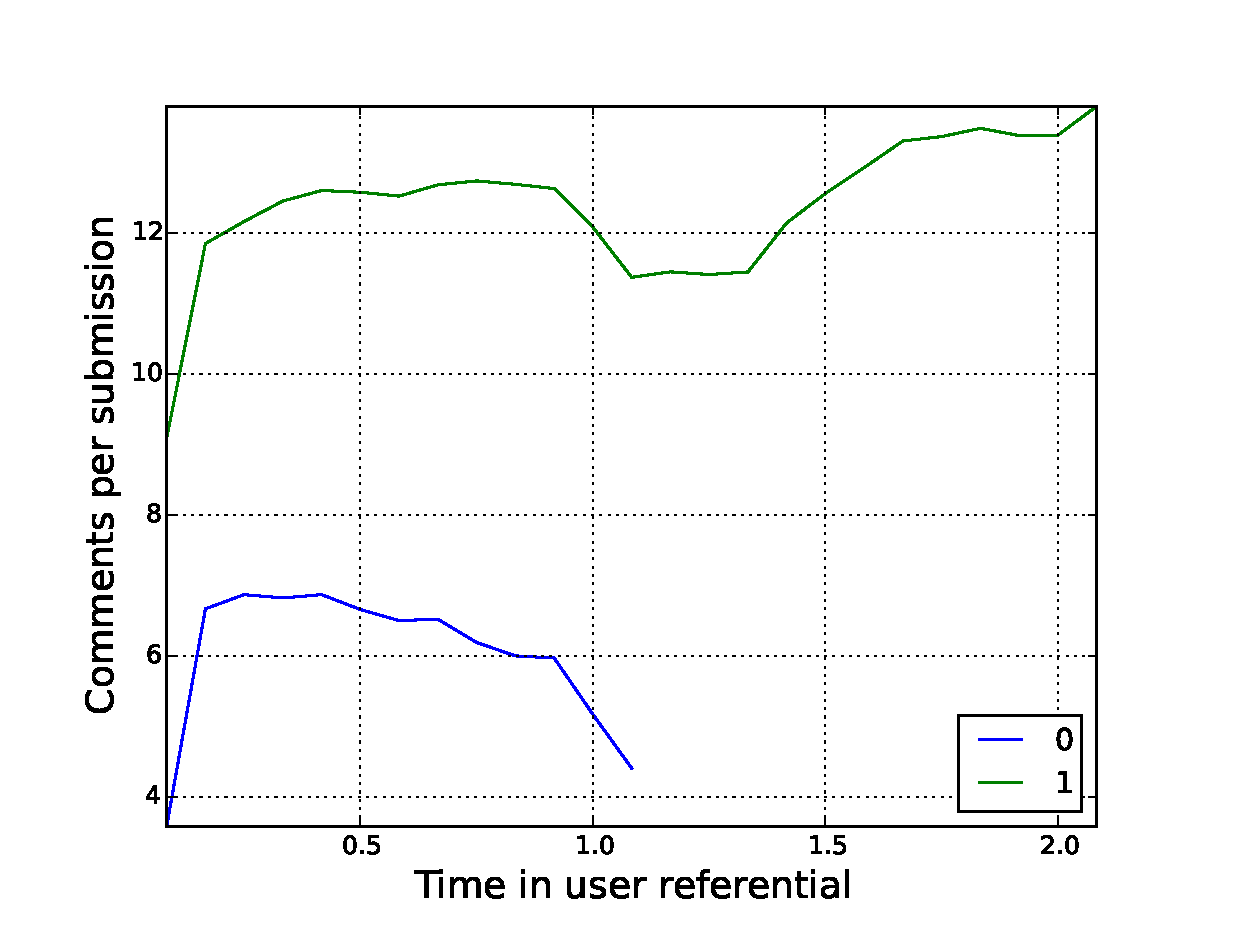
\includegraphics[scale=0.2]{./images/comments_per_submissions_for_surviving_year_for_2013.eps}
\caption{Just as in Figures \ref{fig:avr_posts_per_user_for_surviving_year}, each figure corresponds to one cohort. Each cohort was segmented based on users according to how many years they survived. Each figure show the comment per submission ratio for these groups of users per cohort. We can observe a clear pattern of users that die earlier having a lower comment per submission ratio. Also, these curves do not show clear signs of increase over time, which suggests that the main reason for the cohorted user-referential ratio in Figure \ref{fig:comments_per_submissions_cohorts} to increase is due to the fact that the low performers drop out earlier.}
\label{fig:comments_per_submissions_for_surviving_year}
\end{figure}

\subsection{Users' Effort}

In the previous sections we observed that the average effort per post for older cohorts increases as the users survive in the network. We also observed that users from older cohorts present higher effort per post for the same survived time than users from earlier cohorts. This means that as you age in reddit, you write more per post, and the earlier you joined, the more you write. But we also observed that users from earlier cohorts are commenting more than users from older cohorts for the same time survived in the network. Could users be actually putting the same effort in terms of number of written characters, but younger users do it writing more, shorter posts while older users write less, longer posts? To investigate this, we follow the same steps as in the previous sections, analyzing the overall and cohorted behaviors, over time and from the user time referential.

%% Sam 12: A much better approach to these graphics is to join the overall curve with the cohorted cuves. Not only we save space, but we make the differences in the overall average and the cohorted trends more clear. Will be doing this for all graphics in previous sections, but might not have time to do all of them today.

%\begin{figure}[!tb]
%\centering
%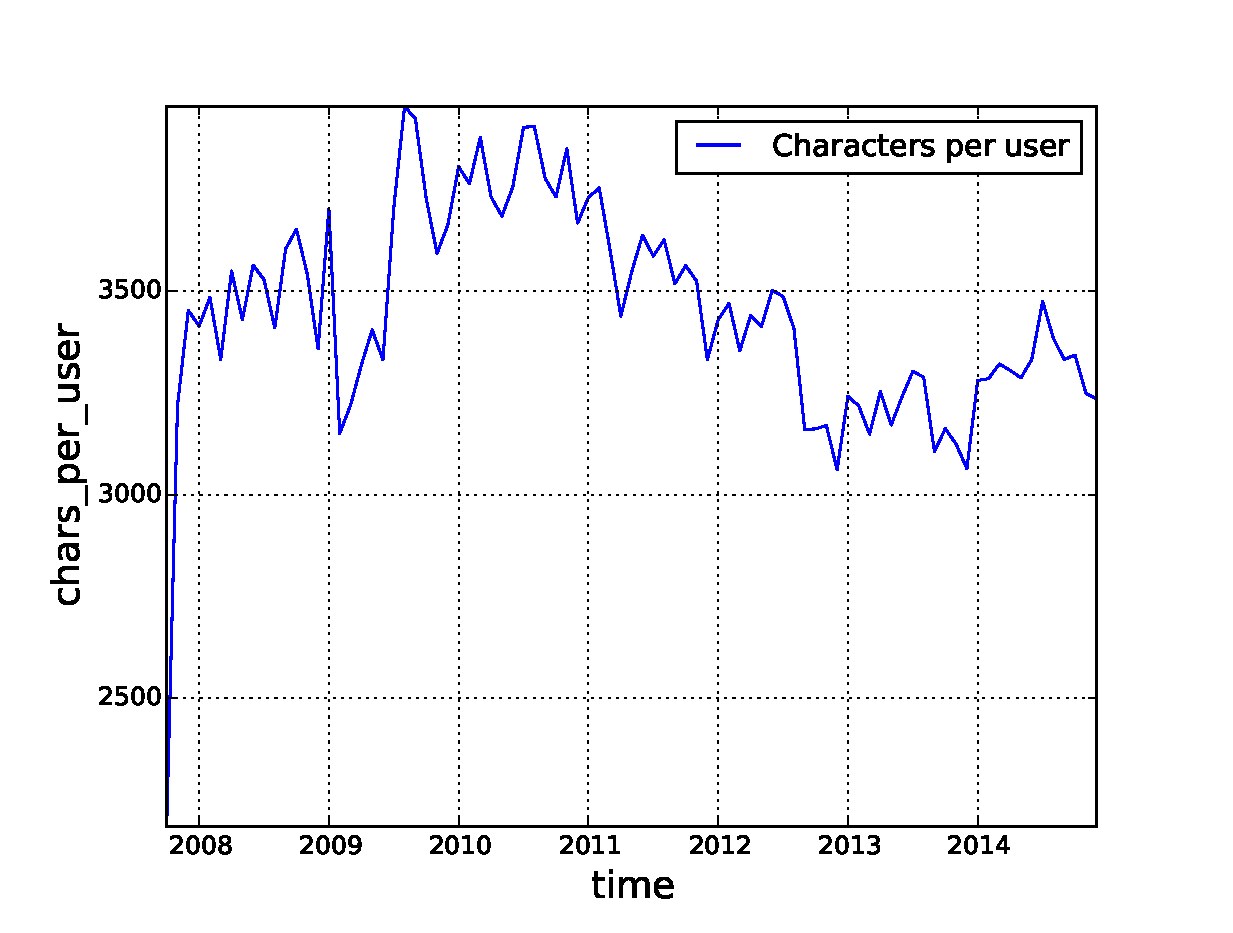
\includegraphics[scale=0.4]{./images/avr_comment_size_user_over_time_total.eps}
%\caption{Average number of written characters per user over time for the reddit network. Here we observe that the average number of characters a user writes per month in reddit had it maximum at around 2010. After that, we observe a slightly decreasing pattern for this proxy for user effort on average in the network.}
%\label{fig:avr_comment_size_user_over_time_total}
%\end{figure}

\begin{figure}[!tb]
\centering
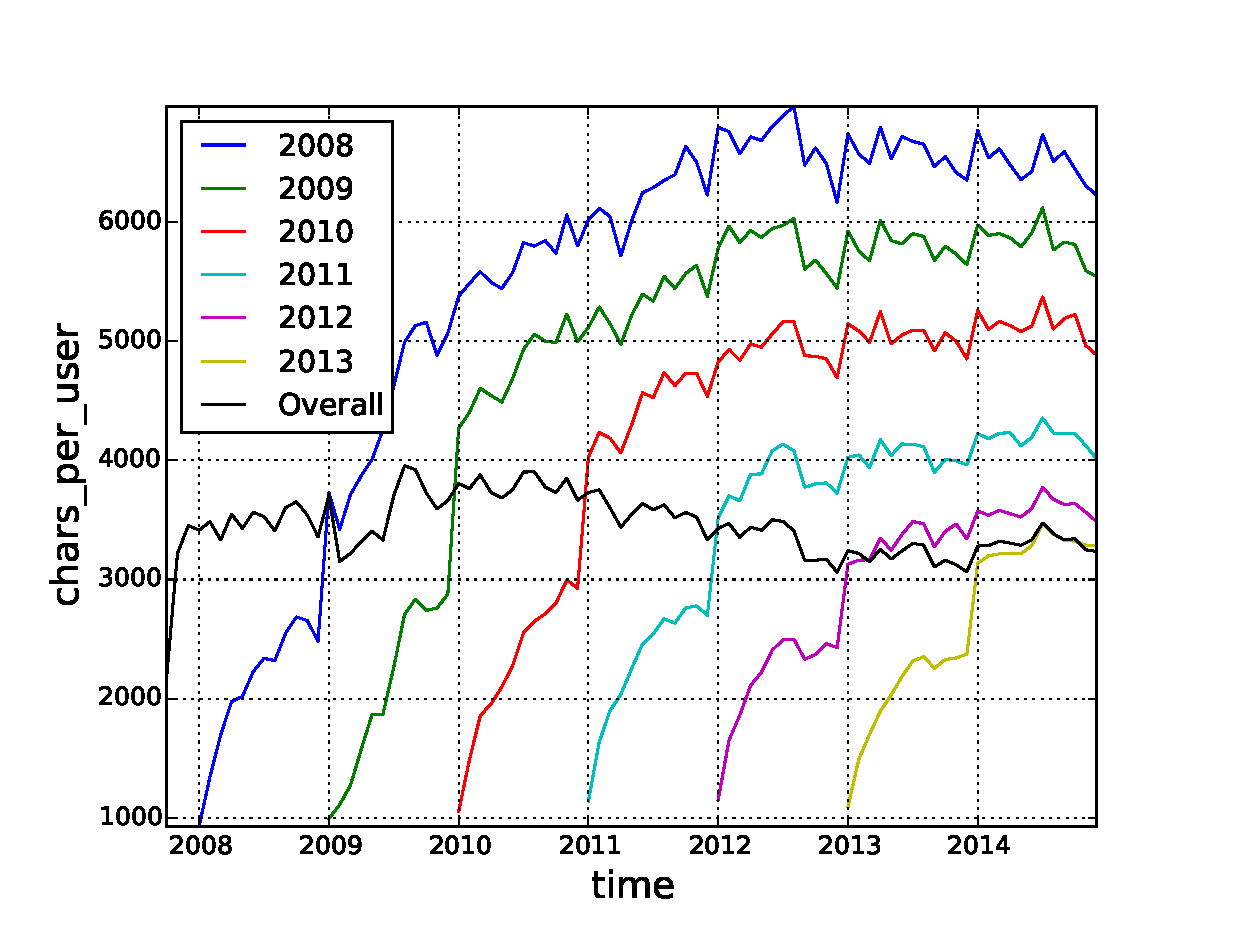
\includegraphics[scale=0.4]{./images/avr_comment_size_user_over_time_cohorts.eps}
\caption{Average number of written characters per user over time for cohorts on user creation time superimposed over the trend for the total of users. The overall average number of characters a user writes per month in reddit for the total of users had it maximum at around 2010. After that, we observe a slightly decreasing pattern for this proxy for user effort on average in the network. We also observe in the cohorted curves that, at any point in time, the average number of characters that older cohort users write per month is always higher than the earlier cohorts. Also, as with other per user averages, these curves are significantly different in the cohort year, since users are being created in the period.}
\label{fig:avr_comment_size_user_over_time_cohorts}
\end{figure}

In Figure \ref{fig:avr_comment_size_user_over_time_cohorts}, we observe that during most of the time, the overall average number of characters written per user per month stays between 3000 and 3500, peaking near 2010 and showing a slightly downwards tendency throughout the end of 2014. The cohorted curves show a different growth pattern in comparison with the overall trend, mainly increasing and then leveling at different values, with older cohorts higher than younger ones. The decreasing overall trend happens because the latter cohorts have a much more significant weight in the average due to the increased number of users that joined reddit in the later years. This highlights the differences of the overall trend for the cohorted trend: while the overall shows a slightly decrease towards 2014, the cohorts show an increasing and leveling behavior. This can lead to wrong conclusions if not treated properly.

%\begin{figure}[!tb]
%\centering
%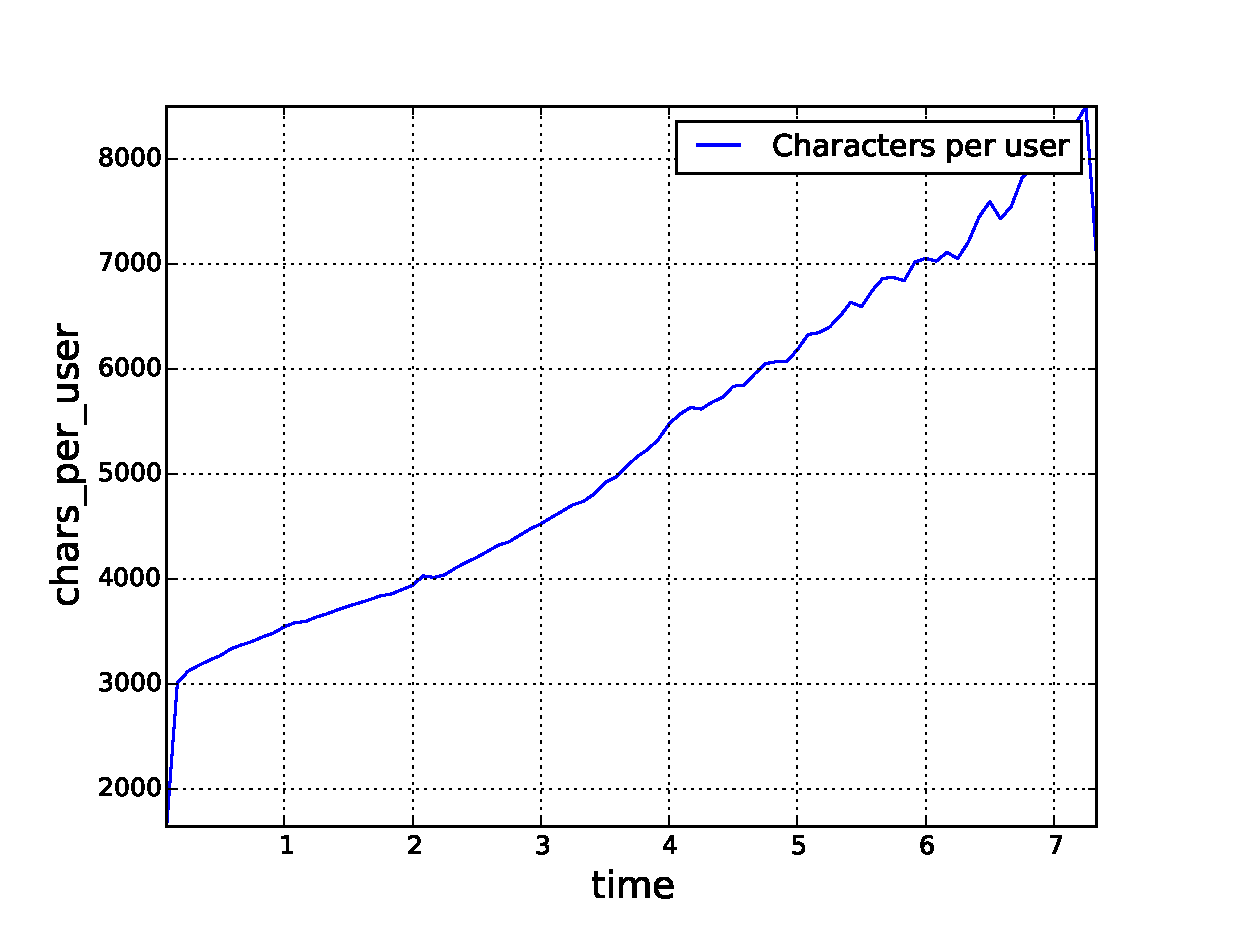
\includegraphics[scale=0.4]{./images/avr_comment_size_user_user_ref_total.eps}
%\caption{Average number of written characters per user from the users time referential. This graphic shows that, as users survive in the network, the number of characters they are likely to write every month increases.}
%\label{fig:avr_comment_size_user_user_ref_total}
%\end{figure}

\begin{figure}[!tb]
\centering
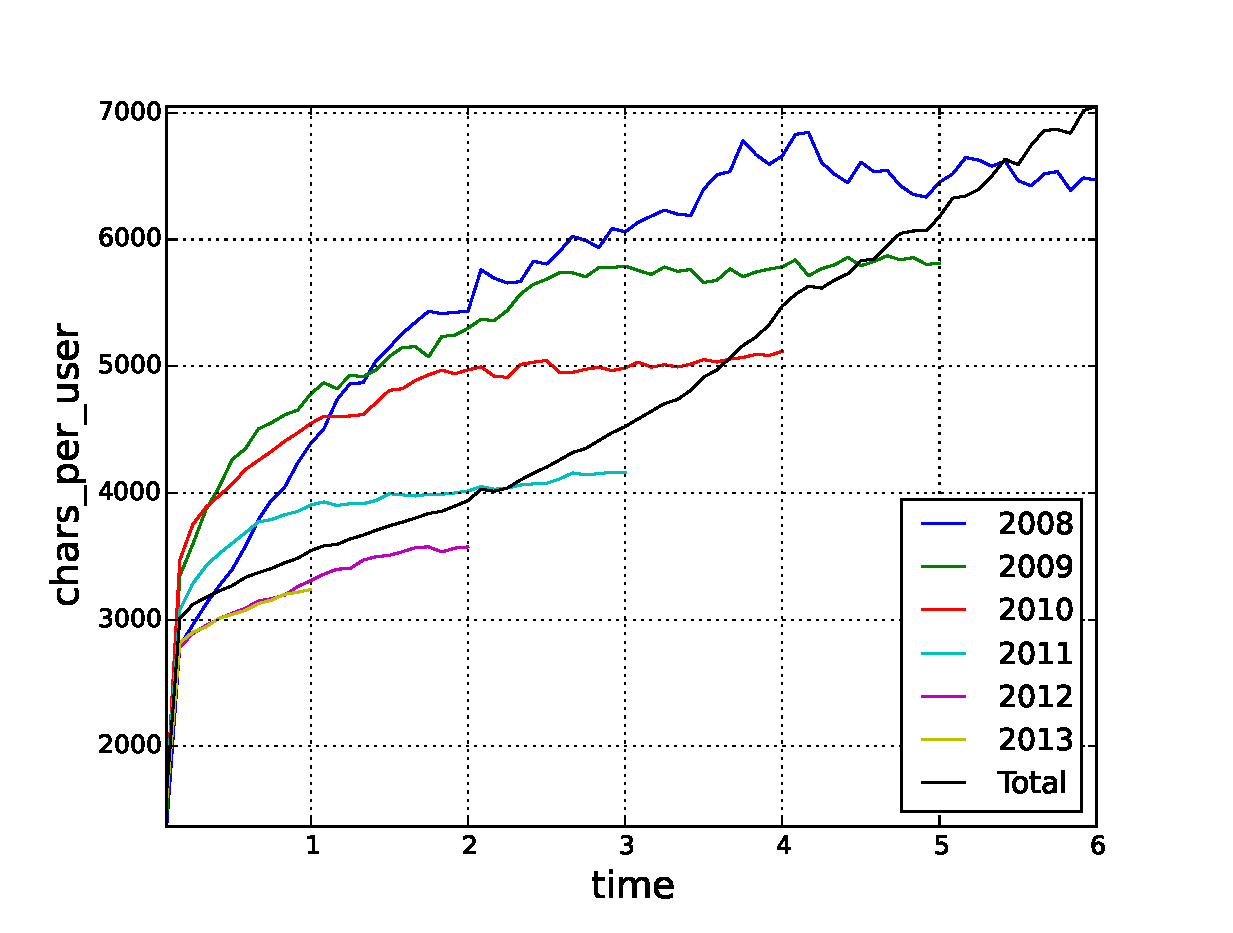
\includegraphics[scale=0.4]{./images/avr_comment_size_user_cohorts.eps}
\caption{Average number of written characters per user from the user time referential segmented by user creation cohorts superimposed with the average number of written characters per user from the users time referential for the total of users in the network. The overall line shows that, as users survive in the network, the number of characters they are likely to write every month increases. We also observe for the cohorted curves that the surviving users level at different values, with a clear general pattern for users in older cohorts to level at higher values than younger ones, given the same time lived in the network. The partial exception is 2008, that presents a lower evolution in the first one and a half year. Since, as in the previous cases, we can not know if this is because users took a longer time to write more of the low-effort users stayed around for a longer time, we have to further segment these cohorts by the time each user existed in the network. It is also important to notice how the shapes of the cohorted curves are different from the total line. This happens because the cohorts have different weights in the total curve because of larger number of users in them.}
\label{fig:avr_comment_size_user_cohorts}
\end{figure}

To further investigate how users evolve in the network, we see in Figure \ref{fig:avr_comment_size_user_cohorts} the number of written characters per month per user from the user time referential for the overall average and the user creation date cohorted curves. We observe a sharp increase in the beginning of all lines due to the fact that a significant number of users only survive a very short time and the total amount of characters they contribute is considerably lower in comparison with the ones that survive for longer. The effect these users have in the analysis is concentrated in the leftmost part of the graphic, which improves the analysis in this referential. We can see that users, as they survive, write more characters per month. This can be due to the fact that users write more as they age and/or because users that write less die first and the surviving ones are the ones that write the most. From the user perspective, we see that the evolution of overall trend and the cohorted ones are significantly different. The overall trend shows a positive second derivative and apparently keep increasing for older users, while the cohorted ones have a negative one and eventually level. The conclusions about how users behave based on this can be quite misleading, specially considering that it is not reasonable for users to be forever increasing the amount of written characters as they survive.

\begin{figure}[!tb]
\centering
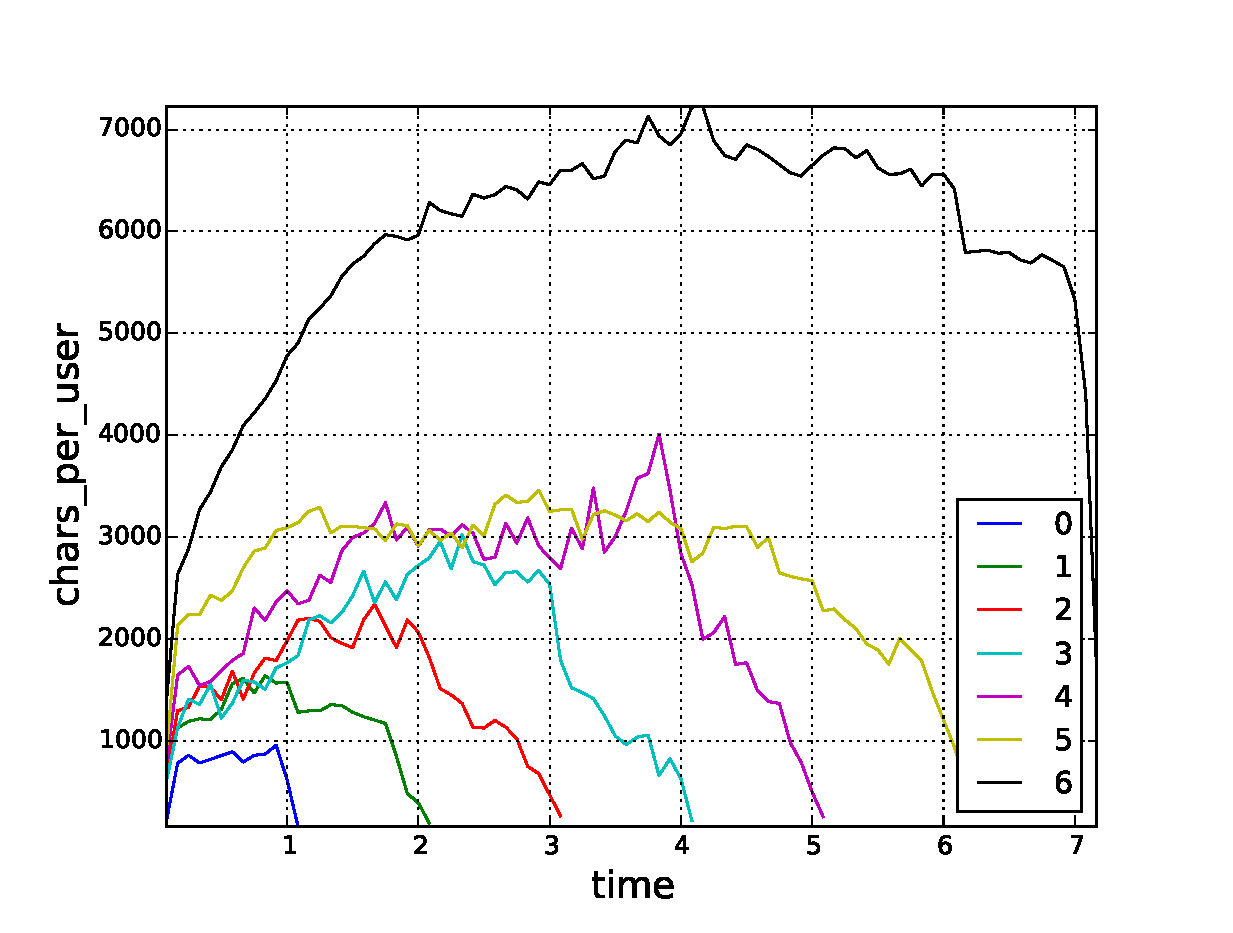
\includegraphics[scale=0.2]{./images/avr_comment_length_user_for_surviving_year_for_2008.eps}
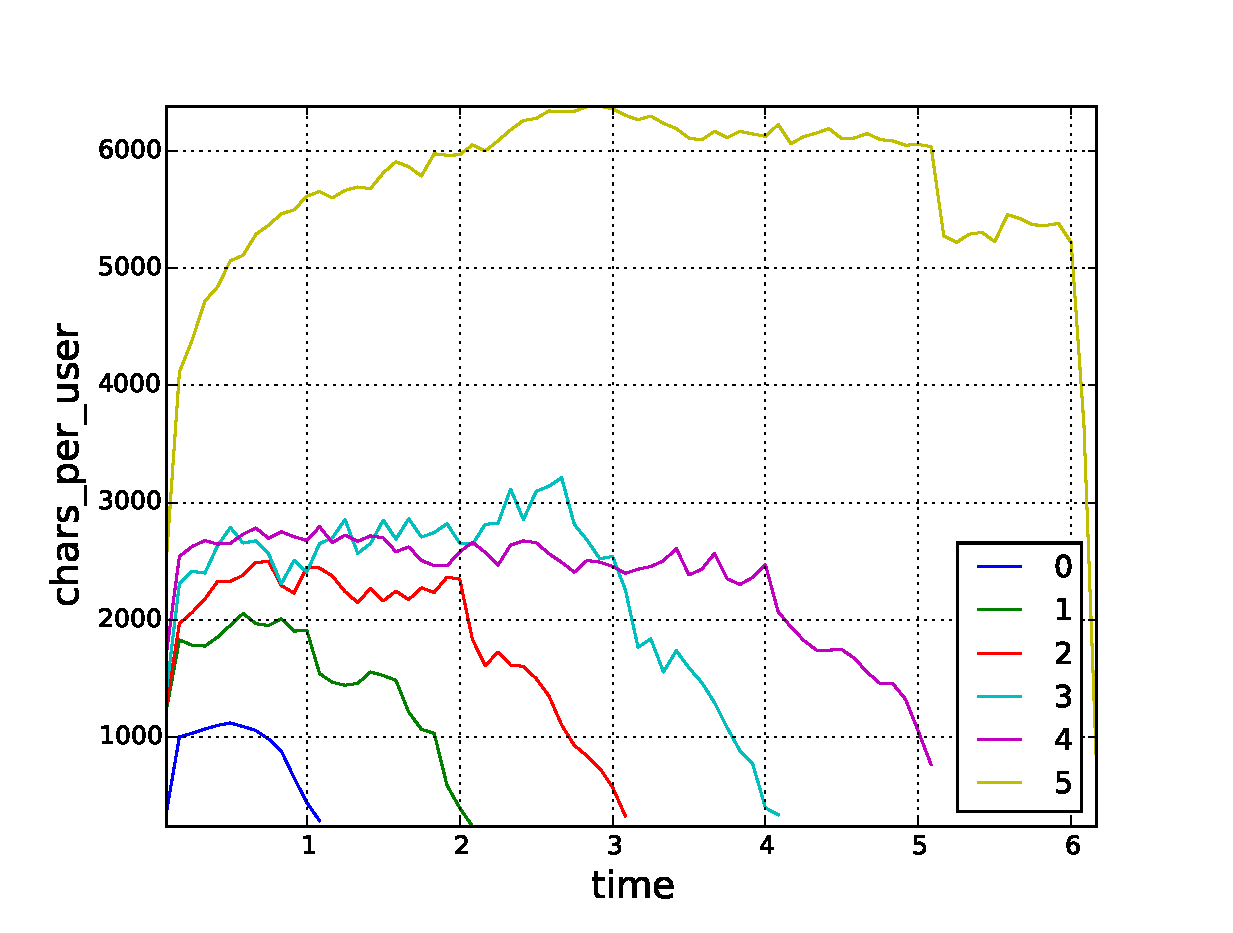
\includegraphics[scale=0.2]{./images/avr_comment_length_user_for_surviving_year_for_2009.eps}
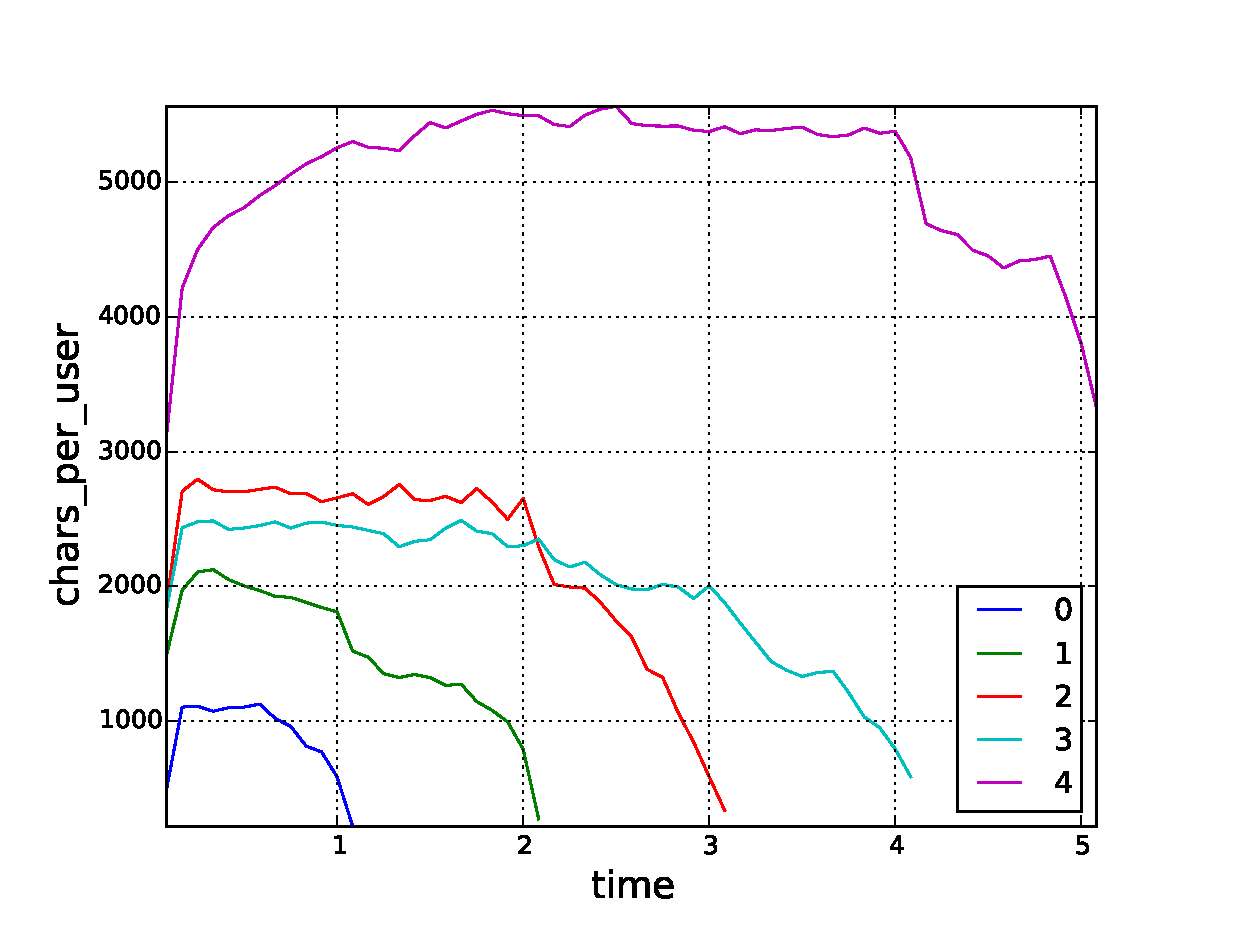
\includegraphics[scale=0.2]{./images/avr_comment_length_user_for_surviving_year_for_2010.eps}
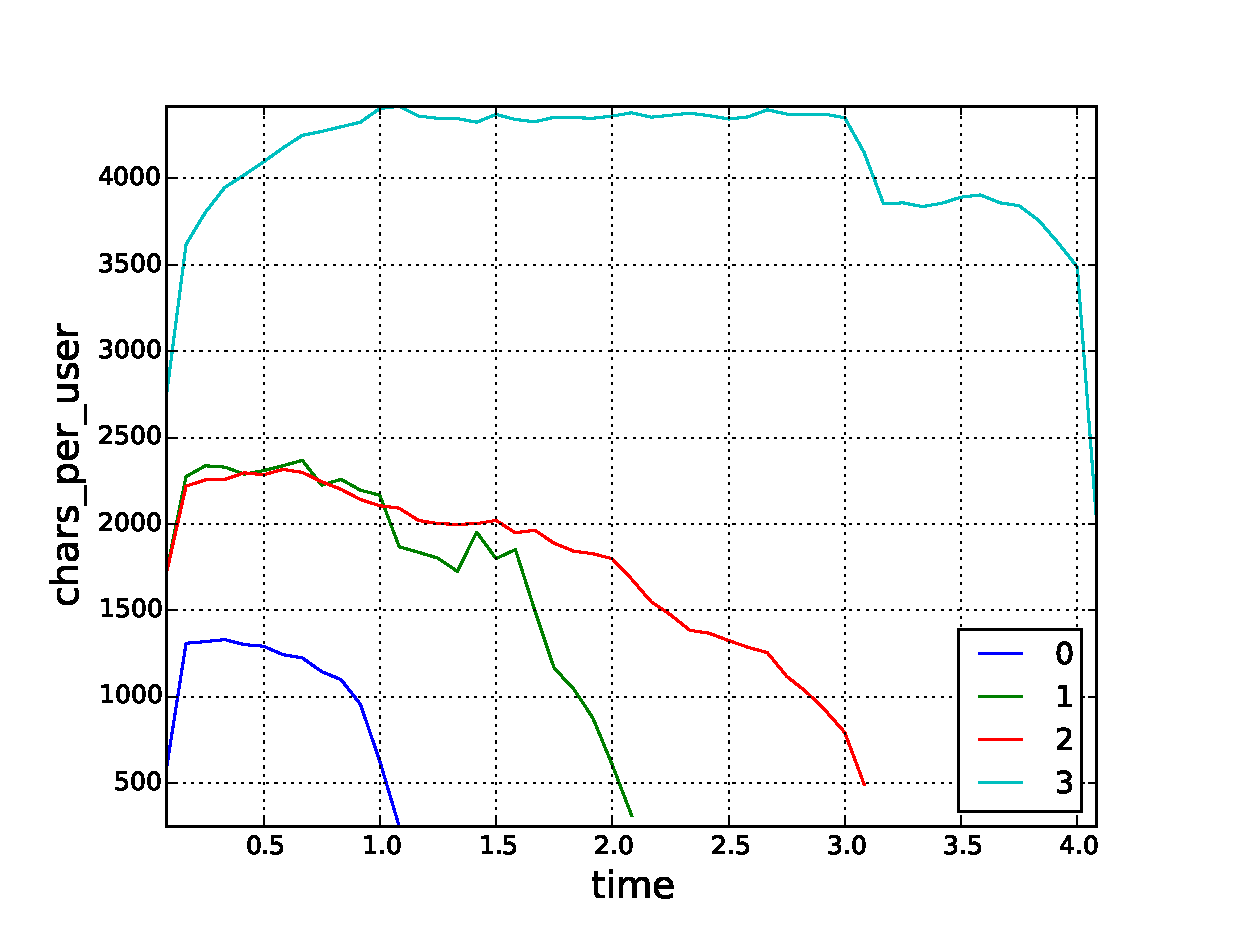
\includegraphics[scale=0.2]{./images/avr_comment_length_user_for_surviving_year_for_2011.eps}
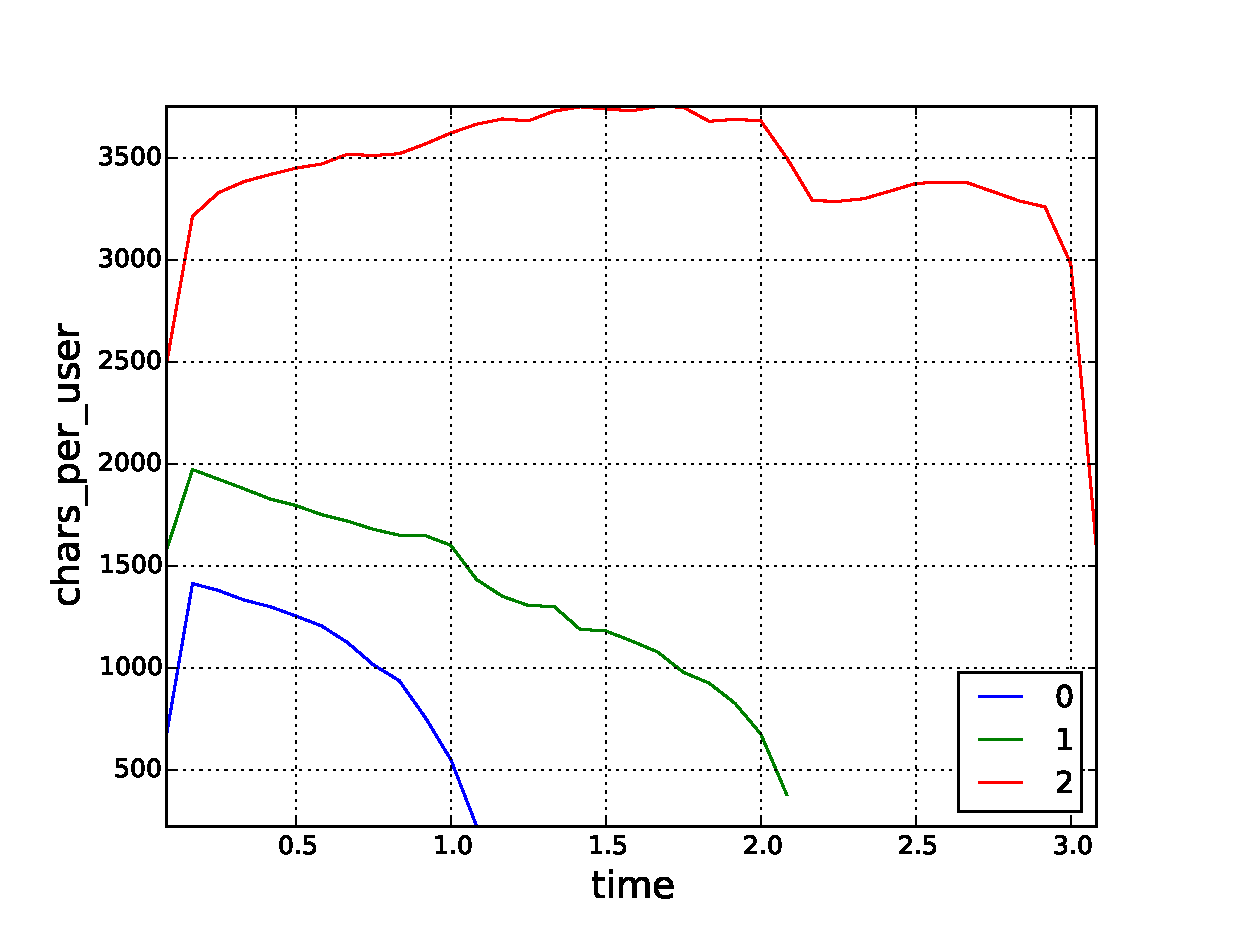
\includegraphics[scale=0.2]{./images/avr_comment_length_user_for_surviving_year_for_2012.eps}
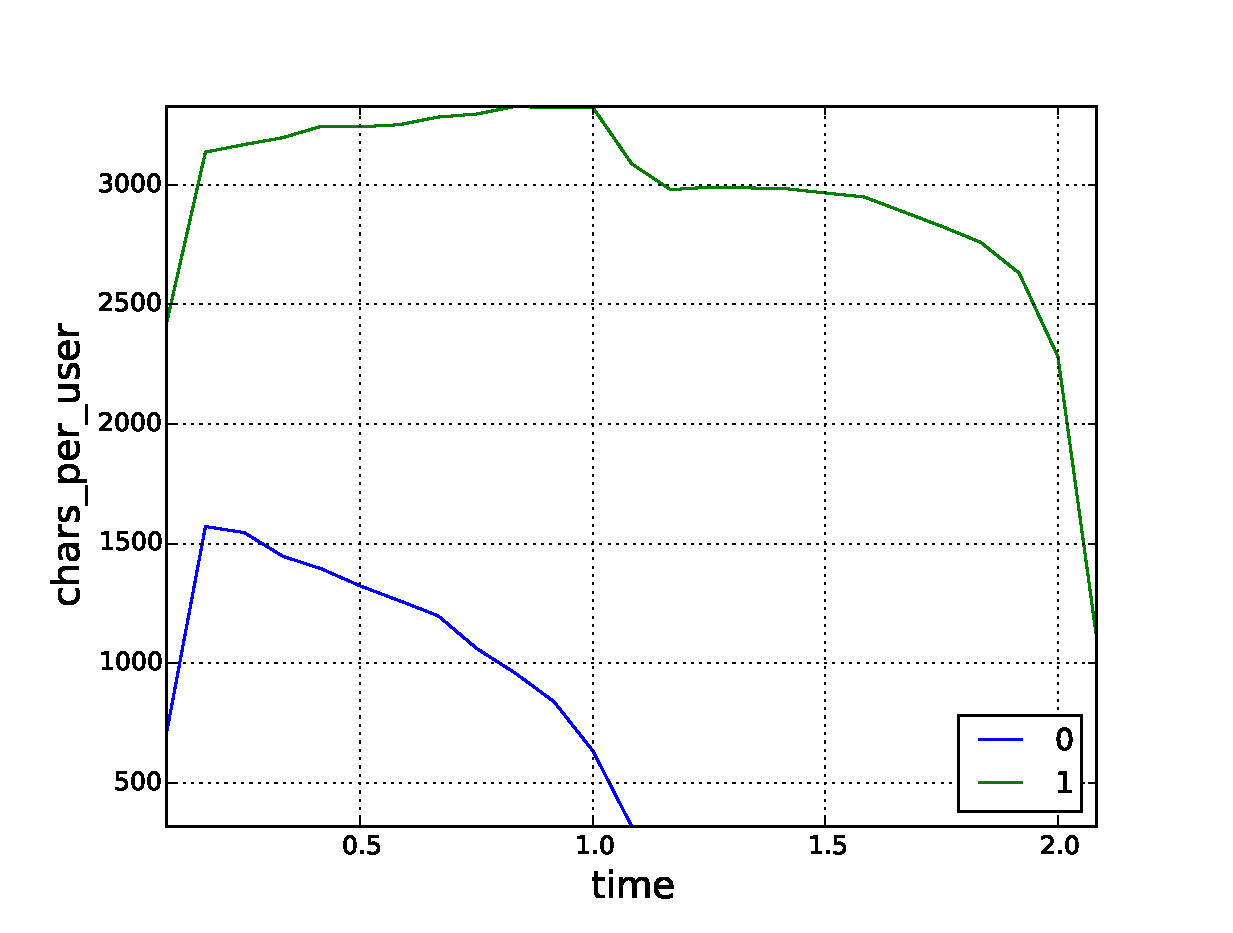
\includegraphics[scale=0.2]{./images/avr_comment_length_user_for_surviving_year_for_2013.eps}
\caption{Just as in Figure \ref{fig:avr_posts_per_user_for_surviving_year}, each figure corresponds to one cohort. These figures show the average number of written characters per user for users segmented by the number of years that he/she survived in the network, given a cohort. Here we observe that users average number of written characters per month tend to level at higher values the longer one individual survive in the network. For the 2008 cohort from Figure \ref{fig:avr_comment_size_user_cohorts}, this shows evidence that the initial lower behavior of the 2008 curve is because the low-effort users did not die as fast as in the latter cohorts. Also, it shows that the main reason for the average user effort increases as users survive is due to the fact that the lower-effort users die faster.}
\label{fig:avr_comment_length_user_for_surviving_year}
\end{figure}

To understand the increasing amount of written characters as the users age in the network, Figure \ref{fig:avr_comment_length_user_for_surviving_year} shows the per cohort set of figures that segments the users in each cohort according to the number of years survived. We can see clear trends of users leveling in different values of written characters per month according to the number of years they are likely to survive. This means that most of the increasing behavior of the user-time referential is due to users that write few characters dying earlier.

\subsection{Users' Survival}

The simplest definition of an active user in reddit is to set a threshold date and define that every user that posted after that date is an active user and users that do not show any kind of behavior are ``dead''. This, however, is a limited interpretation of how users decide to stay or leave the network, specially if we want to analyse how this behavior changed over time. Also, since our users might always come back to the network at a later time, they might be ``reborn'', that means we have right censored data.

To account for these, we look at a one year window of time for each user. This way, we avoid the right censored data and the possibility that a user might have come back to the network at a later time. Given this, we segment users by their cohort and define that users active in the last 3 months of this one year window are active users. Based on this data manipulation, we present the Kaplan-Meier (cite) survival curve in Figure N.

\begin{figure}[!tb]
\centering
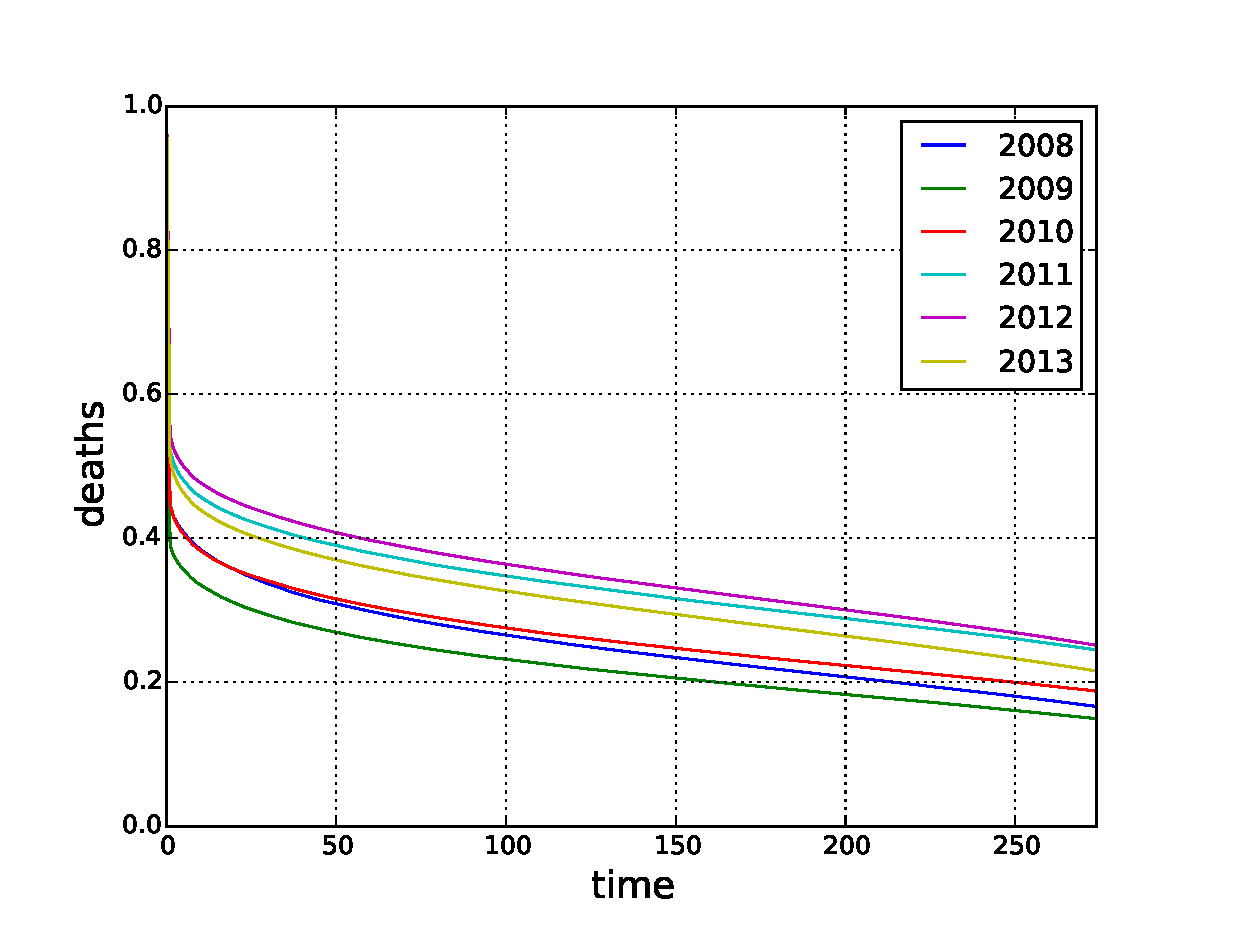
\includegraphics[scale=0.4]{./images/kaplan_meier_users.eps}
\caption{Kaplan-Meier estimator for one year of posting behavior for each user. Users for which the last posting day was in the first nine months of the one year window are considered ``dead''. This graph shows the percentage of surviving users per number of days since it first posted segmented by the cohort year the user joined the network.}
\label{fig:kaplan_meier_users}
\end{figure}

As previously mentioned, reddit shows a significant number of ``single time users'' that only post once in their existence. This can be seen in the initial drop in the first day. An interesting thing to see is that, although different cohorts level in different survival values, the ``user decay'' is similar throughout all of them. Not only that, but there is a general trend for older cohorts to die faster than younger ones. One possible explanation for that is that early reddit still lacked in content, with few subreddits to submit and few submissions to comment. This could lead to a higher number of users that did not stayed around after their initial impressions. 

%% Sam 10: This figure can go if we don't want/can't give a better explanation regarding survival. It is quite common for survival works to have the hazard plot, although I don't fully understand the values myself.
\begin{figure}[!tb]
\centering
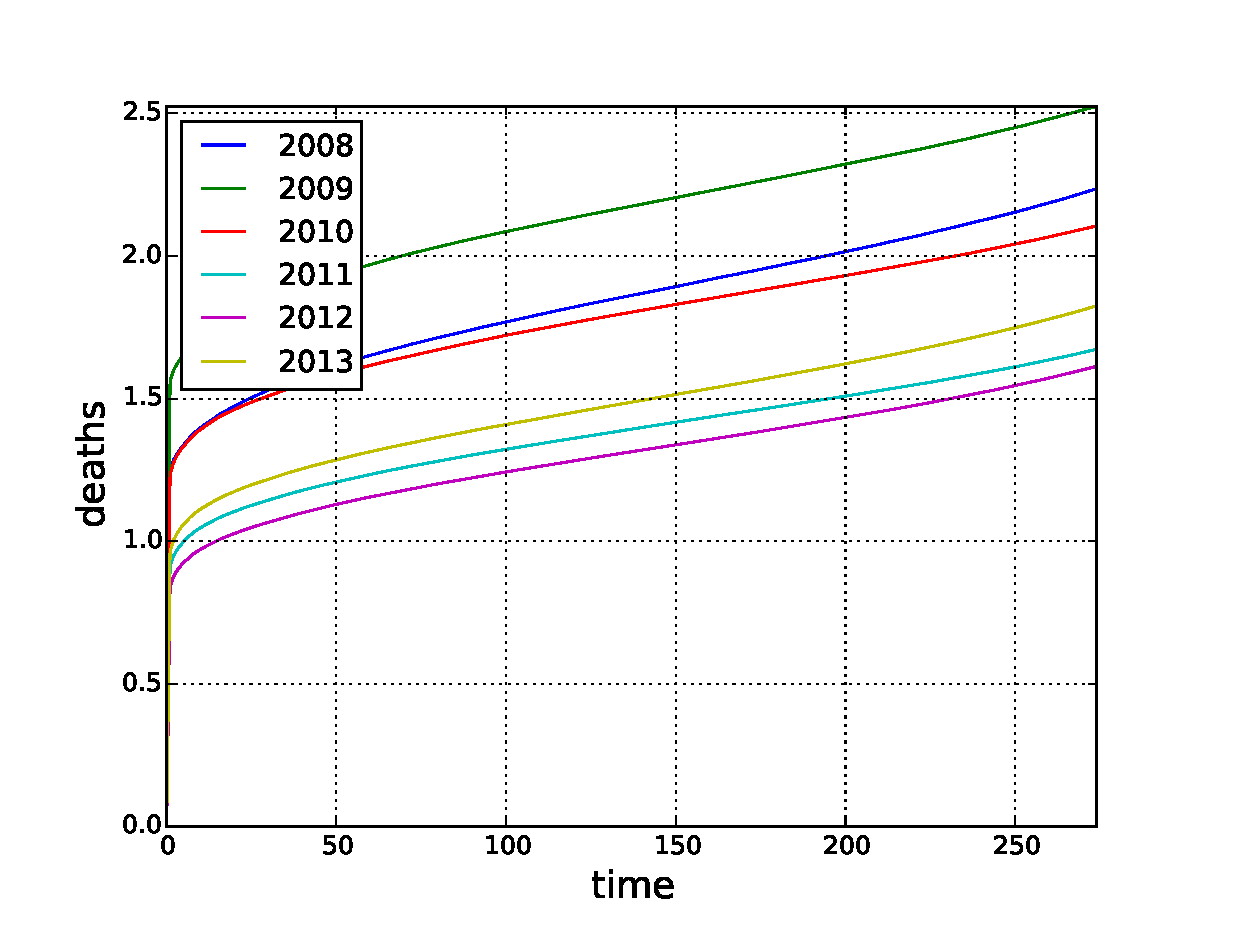
\includegraphics[scale=0.4]{./images/nelson_aalen_users.eps}
\caption{Nelson-Aalen empirical hazard estimation for the users survival. This curves show the pointwise probability of a user to die in time.}
\label{fig:nelson_aalen_users}
\end{figure}
